% Documents settings
\documentclass[twoside]{report}

% Loading configs
% Defining some custom commands here...

% Custom variables
\def\SimWidth{\textwidth}
\def\SchematicWidth{0.7\textwidth}
\def\SmallSchematicWidth{0.24\textwidth}

% Standard paths
\def\Images{images}
\def\Config{config}
\def\Schematics{data/circuitikz}
\def\Drawings{data/tikz}
\def\Timings{data/timings}
\def\Tables{data/tables}
\def\Pdf{data/pdf}
\def\Graphes{data/graphes}
\def\Code{data/code/Opale/application/src}
\def\Conf{data/code/Opale}
\def\DeviceTree{data/code/Opale/boards/topaze/DTSI}
\def\Src{chapters}

% Tikz timings
\usepackage{xparse} % NewDocumentCommand, IfValueTF, IFBooleanTF

% Reference a bus.
%
% Usage:
%
%     \busref[3::0]{C/BE}    ->   C/BE[3::0]
%     \busref*{AD}           ->   AD#
%     \busref*[3::0]{C/BE}   ->   C/BE[3::0]#
%
\NewDocumentCommand{\busref}{som}{\texttt{%
        #3%
        \IfValueTF{#2}{[#2]}{}%
        \IfBooleanTF{#1}{\#}{}%
    }}

% packages
\usepackage{float}
\usepackage{graphicx}
\usepackage{fancyhdr}
\usepackage{subfig}
\usepackage{caption}
% \usepackage[french]{babel}
\usepackage[T1]{fontenc}
\usepackage{hyperref}
\usepackage{minted}
\usepackage{amsmath}
\usemintedstyle{xcode}
\usepackage{placeins}
\usepackage{siunitx}
\usepackage{circuitikz}
\usepackage{pgfplots}
\usepackage{biblatex}
\usepackage{epstopdf}
\usepackage{blindtext}
\usepackage{enumitem}
\usepackage{pdfpages}
\usepackage[	a4paper,
	top=25mm,
	bottom=15mm,
	left=15mm,
	right=15mm,
	head=20mm,
	headsep=5mm]{geometry}
\usepackage[	style=ddmmyyyy,
	yearmonthsep={.},
	monthdaysep={.}]{datetime2}

\usepackage{tikz}
\usepackage{tikz-timing}
\usetikzlibrary{angles,quotes}

\hypersetup{
	colorlinks,
	citecolor=black,
	filecolor=black,
	linkcolor=black,
	urlcolor=black
}

\usetikzlibrary{fit}
\usetikzlibrary{external}
\tikzexternalize

% use the header and footer 
\pagestyle{fancy}

% Document informations
\author{Heywang Léonard - Charles Paolo}
\title{Rapport de TP de Traitement du Signal}
\date{\DTMtoday}

\epstopdfsetup{outdir=./build/\Images/}
\epstopdfsetup{suffix=}


% Document informations
\author{Heywang Léonard, Brandstaedt Arthur}													
\title{Project report : Design of a control system for a small scale rocket}													
\date{\DTMtoday}

% Loading bibtex file
\addbibresource{quote.bib}

% Document
\begin{document}

% Setting font size
\fontsize{9}{10.5}

% Number pages in roman for the introduction (i, ii, iii)
\pagenumbering{roman}

\begin{titlepage}
	\raggedright
	\textbf{Heywang Léonard}	\\
    \textbf{Brandstaedt Arthur}  \\
	Students on the University of Strasbourg, Physics and Engineering departement\\
	1st year of Master in Electronics systems and Microelectronics (SEME).

	\raggedleft
	% Entreprise ...													
	% Addresse
	% Contact	

	\centering
	\vspace{3cm}

	\huge
	\textbf{Projet report : Design of a control system for a small scale rocket}\\
	Semester 1 and 2\\
    \vspace{0.5cm}
	
\includegraphics[width=8cm]{\Images/logo.eps}

	\raggedright
	\normalsize
	\vspace{3cm}
	\textbf{Within the framework of the Master SEME :}\\
	Applied Physics and Engineering, \\
	Electronics systems and Microelectronics

	\vspace{1.5cm}
	\textbf{School year} 2024-2025

	\vspace{1.5cm}
	\textbf{Faculty of Physics and Engineering}\\
	3-5 Rue de l'Université, 67000 Strasbourg\\
	+33 3 68 85 07 30

	\vspace{1 cm}
	\centering
	\begin{figure}[!ht]%
		\centering
		\subfloat{{
\includegraphics[width=5cm]{\Images/logo.eps} }}%
		\qquad
		\subfloat{{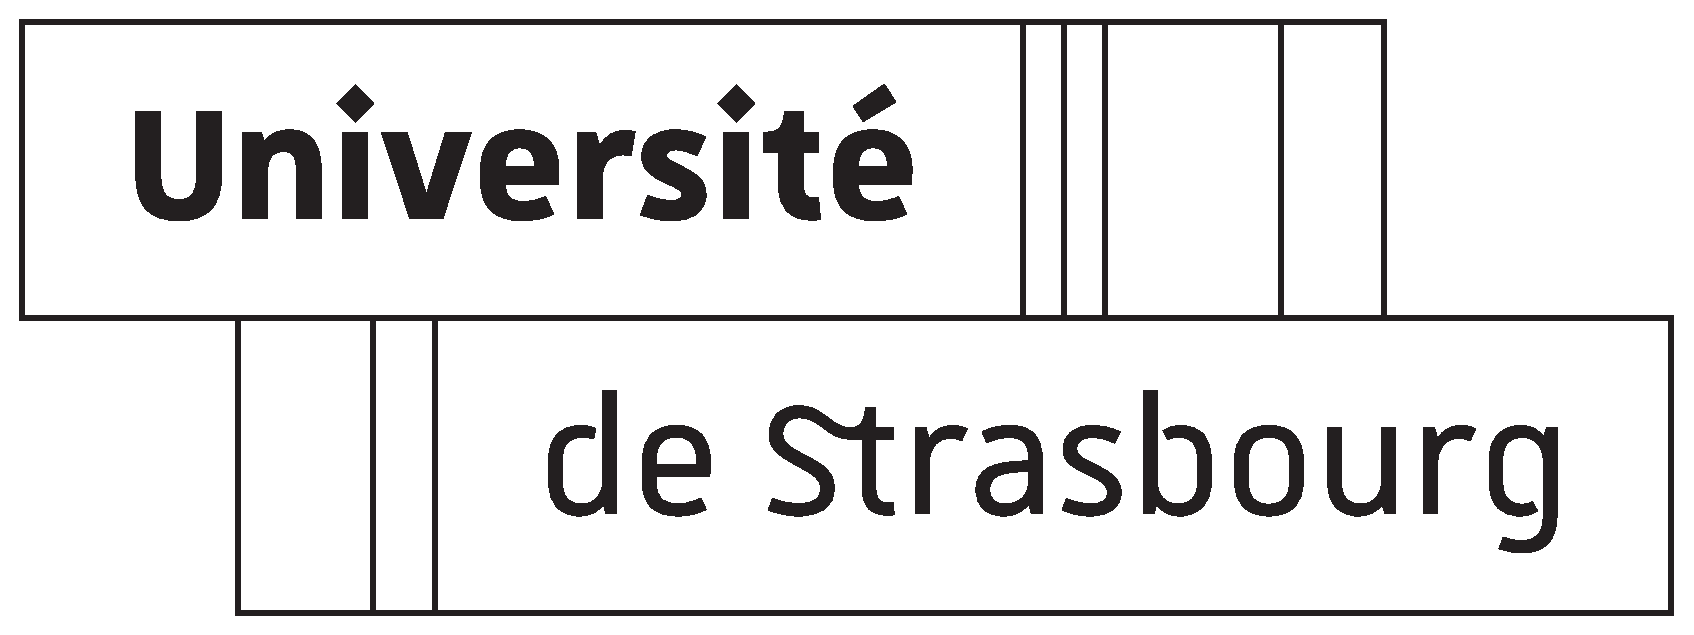
\includegraphics[width=5cm]{\Images/unistra.eps} }}%		
	\end{figure}
\end{titlepage}

% Header and footer definition
\fancyhead{}
\fancyhead[LE, RO]{Project report : Design of a control system for a small scale rocket}
\fancyhead[RE, LO]{
	
\includegraphics[width=3cm]{\Images/logo.eps}
}

\fancyfoot{}
\fancyfoot[CE, CO]{\thepage}
\fancyfoot[RE, LO]{\DTMtoday}
\fancyfoot[LE, RO]{Heywang Léonard - Brandstaedt Arthur}


\tableofcontents
\listoffigures
\listoftables

\newpage
\chapter*{Introduction}
\addcontentsline{toc}{chapter}{Introduction}
\paragraph{}
This document cover the Opale project, which took place in the context inside
the Master SEME on the univeristy of Strasbourg.

\paragraph{}
This project was started on the first semester, by november 2024. The goal was
to develop a small scale rocket that modelize the behavior of real ones. This
model include the usage of powder engines, as well as come control electronics
embedded into the rocket.

This project is named Opale, is making a reference to the french space program
in the 1960s who was using gemstones as rocket model names.
Our control board, the center element of this project is named Topaze, as another
reference of a launcher.

\paragraph{}
For all along this report, we're going to describe all the reflexions, studies,
and conception. Since we're Electronics Engineering students, we'll focus more
on the electronics and sofware aspects, but the mechanical part will also
quicly be explained. The goal with the control electronics is to ensure the
rocket will follow a defined trajectory, as well as storing into an EEPROM some
measurements for an after fly interpretation.

The rocket can be modeled as a complex system, composed with multiple blocks :

\begin{itemize}[noitemsep]
    \item   Sensors (positionning, temperature...)
    \item   Outputs (Servos engines control, engine starter...)
    \item   Controller (MCU + Memory)
    \item   Power supplies
\end{itemize}

\paragraph{}
This report will be splitted in multiple parts, that are not ordered in a
chronological order, but more in a logic way.

\paragraph{}
In the first chapter, we're going to explain how we choosed main hardware
elements, such as the controller, the servo engines or the inertial measurement
unit. These are device where a wide range of choices are possible !

In a second part, we'll focus on the caracterisation of sensors and actuators,
to understand precisely how they behave to any input signals. This is an
important step if we want to develop a precise controller for them !

For a third chapter, we're going to detail the whole procedure of the
electronic design. This start from the schematic, and end up with a whole
printed circuit board, ready to be manufactured.

For the next part, we'll see how we designed the controller of the rocket, from
the physical equations to a simulation, and then implemented into an embedded
controller.

And, to finish the main section, a final part will be dedicated for the whole
software we wrote, that handle the control as well as some other task on the
rocket.

After the conclusion, in annexes there will be some more details. This include
a mechanical overview of the rocket, as well as the process of soldering the
board or some precisions about the software and controller we developped.


\chapter*{System block diagram}
\addcontentsline{toc}{chapter}{System block diagram}
To ensure the reader will understand the following chapters, we drawned a 
block diagram, that summarize most of the important stuff on the project.

\begin{figure}[!hbt]
        \centering
        \resizebox{\SchematicWidth}{!}{%
                \begin{circuitikz}
                        \tikzstyle{every node}=[font=\normalsize]
                        \draw [ fill={rgb,255:red,195; green,232; blue,235} ] (8.75,14.75) rectangle  node {\LARGE MCU + Memory} (17.5,1);
                        \draw [ fill={rgb,255:red,233; green,235; blue,199} ] (2.5,14.75) rectangle  node {\normalsize Sensors } (6.25,8.5);
                        \draw [ fill={rgb,255:red,162; green,199; blue,179} ] (2.5,7.25) rectangle  node {\normalsize Users inputs} (6.25,1);
                        \draw [ fill={rgb,255:red,236; green,195; blue,195} ] (8.75,19.75) rectangle  node {\normalsize Power supplies + Power managements IC (PMIC)} (17.5,17.25);
                        \draw [ fill={rgb,255:red,218; green,187; blue,217} ] (20,14.75) rectangle  node {\normalsize Actuators} (23.75,11);
                        \draw [ fill={rgb,255:red,158; green,148; blue,213} ] (20,9.75) rectangle  node {\normalsize USB Debug port} (23.75,6);
                        \draw [ fill={rgb,255:red,158; green,148; blue,213} ] (20,4.75) rectangle  node {\normalsize User outputs} (23.75,1);
                        \draw [->, >=Stealth] (6.25,4.75) -- (8.75,4.75);
                        \draw [->, >=Stealth] (6.25,11) -- (8.75,11);
                        \draw [->, >=Stealth] (17.5,12.25) -- (20,12.25);
                        \draw [->, >=Stealth] (17.5,8) -- (20.25,8);
                        \draw [->, >=Stealth] (17.5,3.5) -- (20,3.5);
                        \draw [->, >=Stealth] (13,17.25) -- (13,14.75);
                \end{circuitikz}
        }%

        \label{fig:functionnel}
\end{figure}
\newpage

% Set page number in plain numbers (1, 2, 3...)
\pagenumbering{arabic}

\chapter{Component selection}
When starting the project, one of the first points was to choose components.
But, why this one ? And not the other ? Let's dig into the hardware choices we
made here !

\section{Servo engines}
The first component we need to choose were the servo engines. These are
responsible of the position of the wings outside of the rocket. Our criterions
were :
\begin{itemize}
    \item   Minimal error on the control position, ideally with a position feedback.
    \item   Fast enough response.
    \item   Strong enough to resist to the air pressure.
    \item   Small enough to be placed inside of the rocket.
\end{itemize}

We considered the servos listed on the \ref{tab:servo_list} table.

\begin{table}[!hbt]
    \centering
    \begin{tabular}{| c || c | c | c |}
    \hline
    Reference &  Supply voltage & Position feedback & Dimensions (L x W x H)\\
    \hline
    \hline
    LEX-SERVO02 & 4.8 \si{\volt} - 6 \si{\volt} & Yes & 22 \si{\milli\meter} x 12.5 \si{\milli\meter} x 27.3 \si{\milli\meter} \\
    TinyMG 65122 & 4.8 \si{\volt} - 6 \si{\volt} & No & 30 \si{\milli\meter} x 15 \si{\milli\meter} x 30 \si{\milli\meter} \\
    KPower 9g MM090 & 4.8 \si{\volt} - 6 \si{\volt} & Yes & 22.4 \si{\milli\meter} x 12.5 \si{\milli\meter} x 22.8 \si{\milli\meter} \\
    FEETECH FT3325M & 4.8 \si{\volt} - 6 \si{\volt} & No & 30 \si{\milli\meter} x 10 \si{\milli\meter} x 35.5 \si{\milli\meter} \\
    FEETECH FT1117M & 4.8 \si{\volt} - 6 \si{\volt} & Yes & 22 \si{\milli\meter} x 12.5 \si{\milli\meter} x 27.3 \si{\milli\meter} \\
    Hitec HS85BB & 4.8 \si{\volt} - 6 \si{\volt} & No & 28 \si{\milli\meter} x 13 \si{\milli\meter} x 30 \si{\milli\meter} \\
    Datan S1123 & 4.8 \si{\volt} - 6 \si{\volt} & Yes & 32.7 \si{\milli\meter} x 15.7 \si{\milli\meter} x 31.7 \si{\milli\meter} \\
    \hline
    \end{tabular}
    \caption{List of the possibles servo engines}
    \label{tab:servo_list}
\end{table}

Our selection end up on the KPower servo engine, because of their availabily on
well known retailers and specs that are enough for our needs.

\section{MCUs}
The second component that required a bit selection was the MCU, the
microcontroller that will control everything. We didn't needed a ton of
computing power, but we needed some advanced peripherals, and eventually an 2.4
GHz radio interface for a remote Bluetooth control.

We considered these MCUs, listed on the \ref{tab:mcu_list} table

\begin{table}[!hbt]
    \centering
    \begin{tabular}{| c || c | c | c |}
    \hline
    Reference &  Supply voltage & Position feedback & Dimensions (L x W x H)\\
    \hline
    \hline
    LEX-SERVO02 & 4.8 \si{\volt} - 6 \si{\volt} & Yes & 22 \si{\milli\meter} x 12.5 \si{\milli\meter} x 27.3 \si{\milli\meter} \\
    TinyMG 65122 & 4.8 \si{\volt} - 6 \si{\volt} & No & 30 \si{\milli\meter} x 15 \si{\milli\meter} x 30 \si{\milli\meter} \\
    KPower 9g MM090 & 4.8 \si{\volt} - 6 \si{\volt} & Yes & 22.4 \si{\milli\meter} x 12.5 \si{\milli\meter} x 22.8 \si{\milli\meter} \\
    FEETECH FT3325M & 4.8 \si{\volt} - 6 \si{\volt} & No & 30 \si{\milli\meter} x 10 \si{\milli\meter} x 35.5 \si{\milli\meter} \\
    FEETECH FT1117M & 4.8 \si{\volt} - 6 \si{\volt} & Yes & 22 \si{\milli\meter} x 12.5 \si{\milli\meter} x 27.3 \si{\milli\meter} \\
    Hitec HS85BB & 4.8 \si{\volt} - 6 \si{\volt} & No & 28 \si{\milli\meter} x 13 \si{\milli\meter} x 30 \si{\milli\meter} \\
    Datan S1123 & 4.8 \si{\volt} - 6 \si{\volt} & Yes & 32.7 \si{\milli\meter} x 15.7 \si{\milli\meter} x 31.7 \si{\milli\meter} \\
    \hline
    \end{tabular}
    \caption{List of the possibles servo engines}
    \label{tab:servo_list}
\end{table}

Our choice end up on the nRF5340 IC, because it has enough computing power for
our need (and it has two cores !) and some advanced peripherals interconnects
(such as PPI, which enable us to connect peripherals between them to create
logic conditions !). But there where another fact : It has an excellent
software support and documentation, which are going to help us a lot. That was
mainly this point that make us select this chip, compared to the other options
which where less documented.

\section{Sensors selection}
The sensors are also an important part of the rocket, because they're the entry
of informations. They thus need to be precise enough, but, more importantly, do
not derive excessively.

And, since these sensors are mostly accelerometers, the cost for these can
easily become important. For this selection, we did had a choice between two
options :

\subsection{A Pair of accelerometers}
A single accelerometer isn't an expensive device, so it's perfectly possible to
use two or more of them on a single board.

And, with some software treatement we can get the position, speed and rotations
of the rocket with only two of them, by derivating the acceleration.

But, this first solution has a major flaw : It will drift over time, leading to
imprecise calculations, and thus : An error. However, this solution may be
viable for slowest devices.

\subsection{An integrated IMU}
To counter this aspect, we selected a more complex device, that integrate
multiple sensors into one. It enable the device to compensate the drift of a
device with another, but there is a cost : This require a complex software.

Hopefully, this software is already integrated into the chip, leaving us with
already treated data.

That's why we choosed the BNO055, an IMU rather than a pair of accelerometers.
Nonetheless, we deciced to implement both options on the board, to let us some
freedom about or solutions, and to tests different possibilites.

\chapter{Caracterisation and measures of actuators}
One of the first steps on this project was to fetch the maximal amount of
informations about the different sensors and actuator we could. Many of this
data is given by the datasheet, and the work to validate is minor, but there is
case where the datasheet didn't provide enough data. This forced us to measure
our custom data.

We're using three elements in that situation :
\begin{itemize}[noitemsep]
    \item The servo engines
    \item The wings
    \item The internal ADC of the MCU
\end{itemize}

Two of them are electrical devices and can easily be characterized. We're now
going to show some of this data :

\section{Characterization of the servo engines}
First, we need to measure precisely how the engines respond to any arbitrary input, to design they're own control loop.
To measure the servo response, we proceeded in two times : A first session, with some electronic specialized tool,
and a second session with the MCU as controller and measuring unit !

\paragraph{}
We used this schematic for the measures :
\begin{figure}[!hbt]
    \centering
    \resizebox{\SchematicWidth}{!}{%
        \begin{circuitikz}
            % ---------------------------------------------------------------------------
            % Draw components
            % ---------------------------------------------------------------------------
            \draw (0,0) node[ground] {} to[vsourcesquare, label=\(V_{\text{PWM}}\)] (0,2) node[] () {};
            \draw (4,2) node[elmech](motor){M};
            \draw (4,0) node[ground] {};
            \draw (4,4) node[vcc] {\(V_{\text{CC}} = 5 \si{\volt}\)};
            \draw (8,2) node[oscopeshape] (osc1) {};
            \draw (2,1) node[oscopeshape] (osc2) {};

            % ---------------------------------------------------------------------------
            % Draw wires
            % ---------------------------------------------------------------------------
            \draw (0,2) -- (motor.left);
            \draw (4,0) -- (motor.bottom);
            \draw (4,4) -- (motor.top);
            \draw (motor.right) -- (osc1.left);
            \draw (osc2.left) -- ++(-0.5, 0) -- ++(0,1) node[circ] {};

        \end{circuitikz}}

    \caption{Schematic used for testing response of servo engines}
    \label{fig:Servo_test}
\end{figure}

\paragraph{}
For the first session, we sent the control signal using a dedicated signal generator, configured
to output a PWM at a frequency of $50 \si{\hertz}$ and with a pulse length between $1 \si{ms}$ and
$2 \si{ms}$.
We measured the output of the servo engines, which is an analog output that reflect the servo position
using an oscilloscope.

\begin{figure}[!hbt]
    \centering
    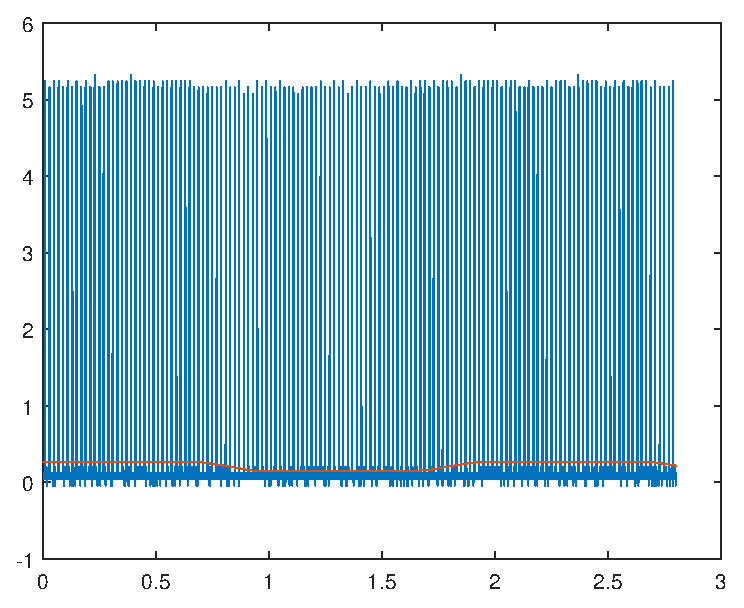
\includegraphics[width=\SchematicWidth]{\Images/Servos/time-domain-response.eps}
    \caption{Time domain servo response}
\end{figure}
\FloatBarrier

\paragraph{}
We can see on this image... nothing ! That's because the pulse length if near 0 compared to the whole
period. And even then, the servo response is quite slow, thus we need a long measure time !

To exploit this data, we used the Matlab "DutyCycle" function, that return the actual duty cycle of a signal.
This gave us results that where ok, but clearly perfectibles :

\begin{figure}[!hbt]
    \centering
    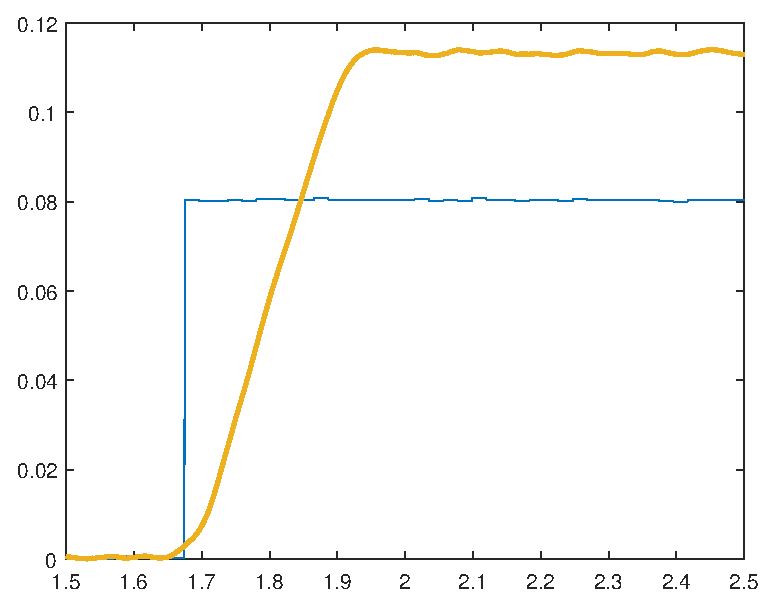
\includegraphics[width=\SchematicWidth]{\Images/Servos/Duty-Forced.eps}
    \caption{Time domain servo response, expressed in duty cycle}
\end{figure}
\FloatBarrier

\paragraph{}
Now, we have a command and a response that seem plausible, except one details : The servo seems to start
\textit{before} the command. That's typically the case for a non-causal systems, which can't be easily controlled,
if at all !
Luckily, in our case this is an issue from the code that draw theses graphes, rathers than the servo by itself.
We used a script that convert the raw measures to theses ones, but there was a bug, which cause this lag \footnote{
    To be precise, the DutyCycle function return a list of n elements, where n is the number of period. We then
    extended this list to match the original lenght. And since the DutyCycle return the value at the end of the
    period, there is $Te$ retard. Thus, a $\frac{1}{Te}$ period is now $\frac{n}{Te}$.
    Combine both, and you end up with a visually non-causal system.
}.

\paragraph{}
Anyway, theses measures weren't that good, they gave a first order approximation but didn't represented
correctly the signal. This was caused by multiple points :

\begin{itemize}
    \item Error on the signal generator : When working at this kind of low frequencies, the signal is quite imprecise.
    \item Too big amplitude on the command. This lead to results that are outisde the interresting range.
\end{itemize}

\paragraph{}
We addressed most of theses points on the second session of measure, where we used the final MCU to control the servos.
We thus got a precise (Up to $\pm 1 \si{\mu\second}$) pulses, and the definitive measure device (the integrated ADC)\footnote{
    Which was already characterized at this point, but, for clarity reasons is explicited in the next section
}.

We got theses measures :

\begin{figure}[!hbt]
    \centering
    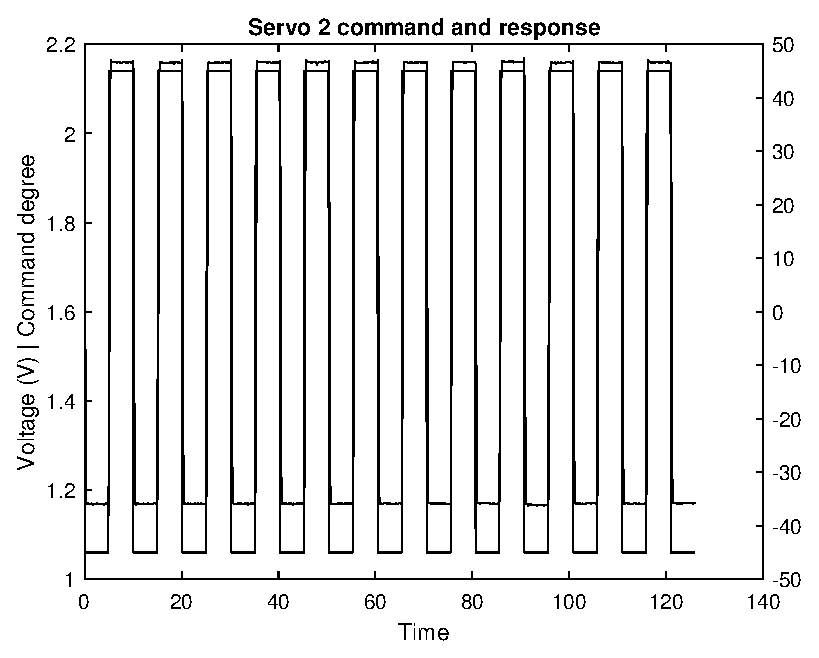
\includegraphics[width=\SchematicWidth]{\Images/Servos/reduced-square.eps}
    \caption{Time domain servo response, expressed in duty cycle}
\end{figure}
\begin{figure}[!hbt]
    \centering
    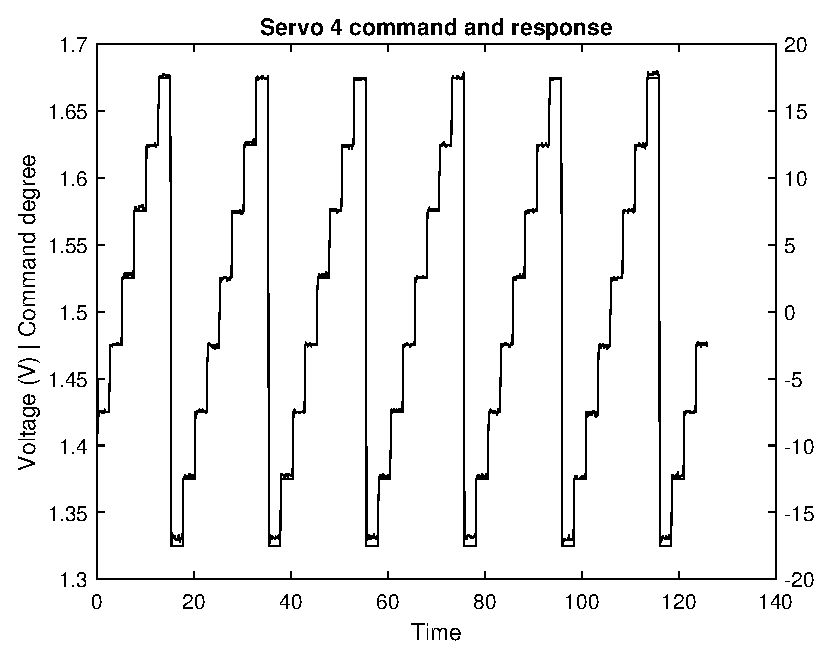
\includegraphics[width=\SchematicWidth]{\Images/Servos/ramp.eps}
    \caption{Time domain servo response, expressed in duty cycle}
\end{figure}
\FloatBarrier

\paragraph{}
Theses are way better than we got on the first session, because we addresses the issues.

Using the zoom functions, we can identify that in our case, the servos engines are responsing
as a very simple device : A first order one.

They goes into the required position in about $1 Te$, which is on our system arround
$120 \si{\milli\second}$ by achieving a linear transition.



\section{Characterization of the ADC}
To conclude this part, let's talk about ADC deviations :

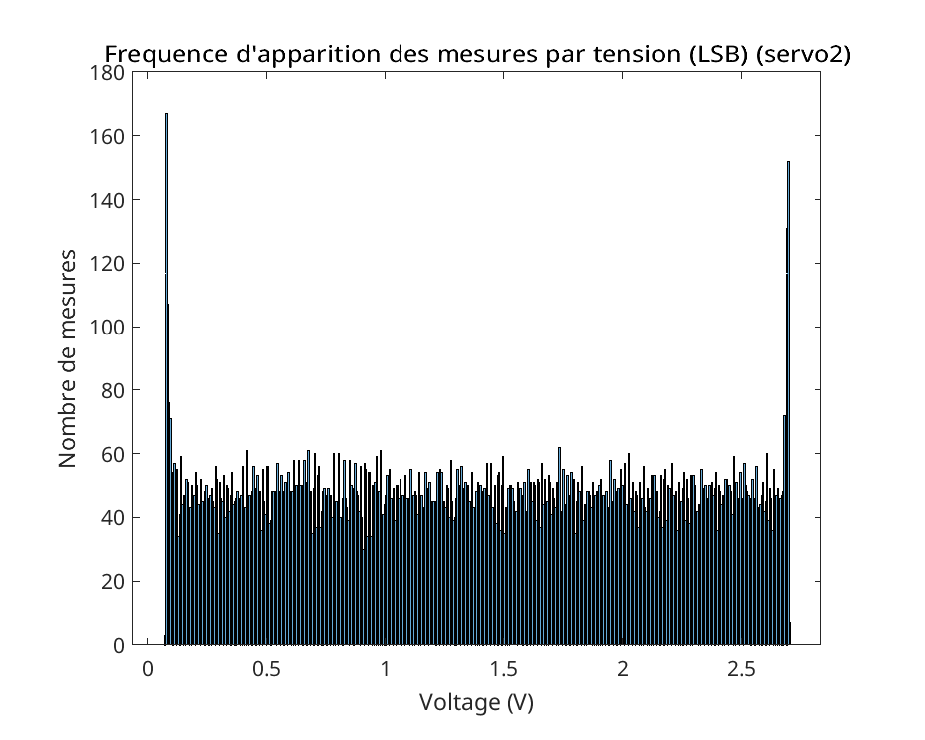
\includegraphics[width=\SchematicWidth]{images/ADC/ADC-DNL.eps}

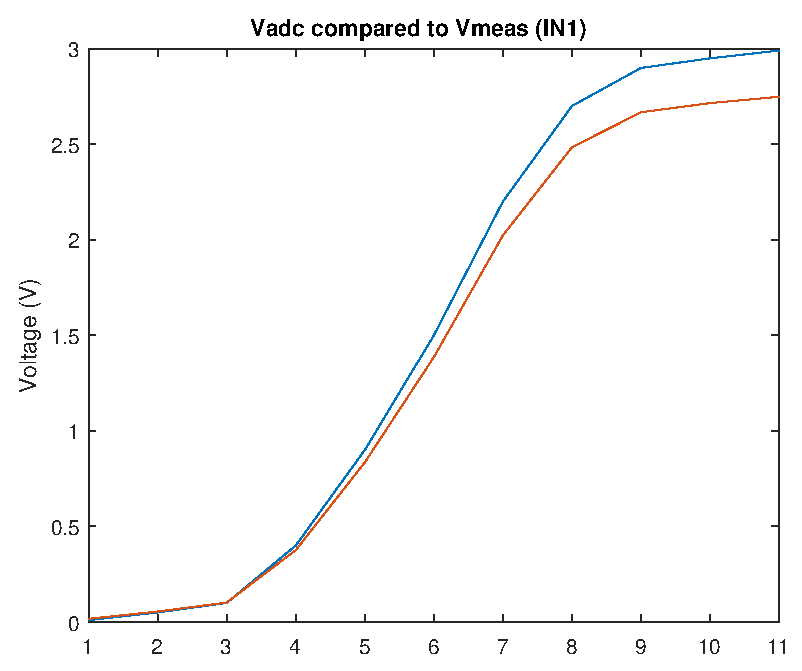
\includegraphics[width=\SchematicWidth]{images/ADC/gain-error.eps}

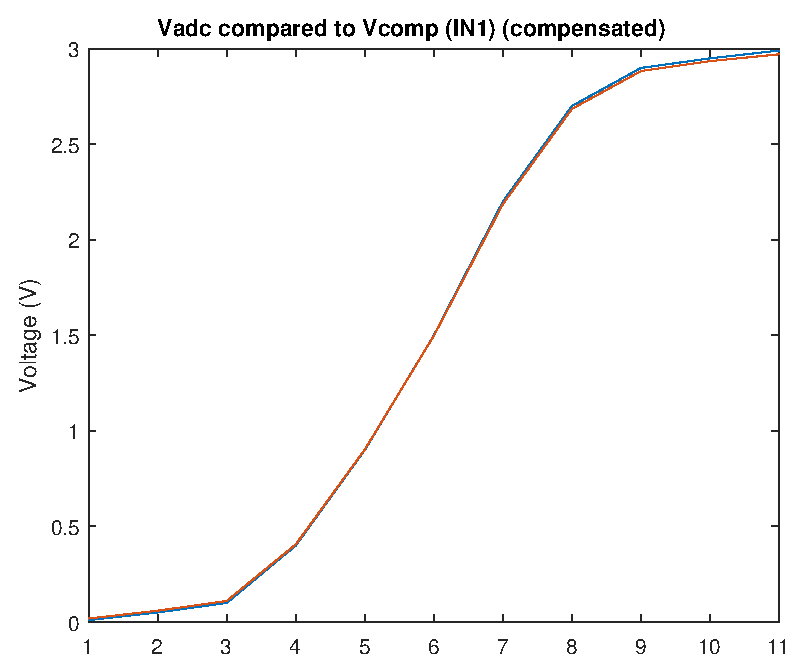
\includegraphics[width=\SchematicWidth]{images/ADC/gain-compensated.eps}

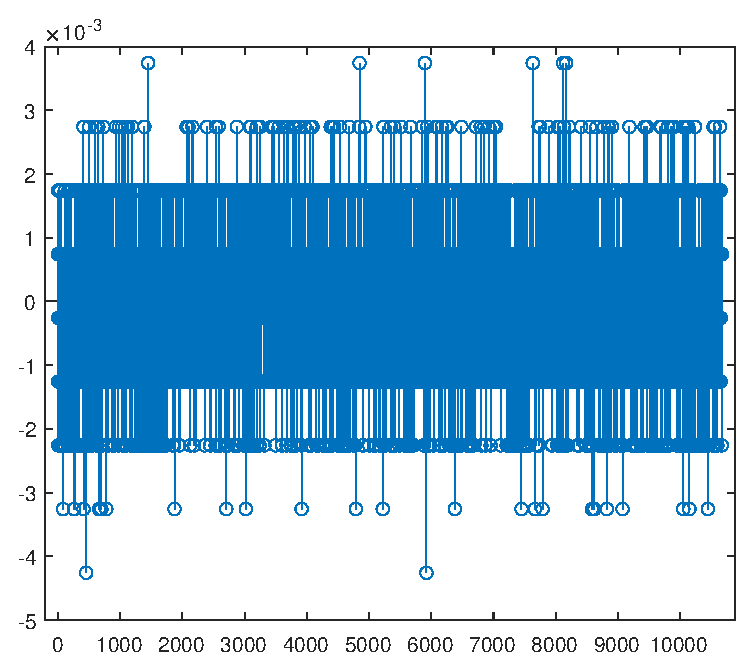
\includegraphics[width=\SchematicWidth]{images/ADC/stdev-adc.eps}

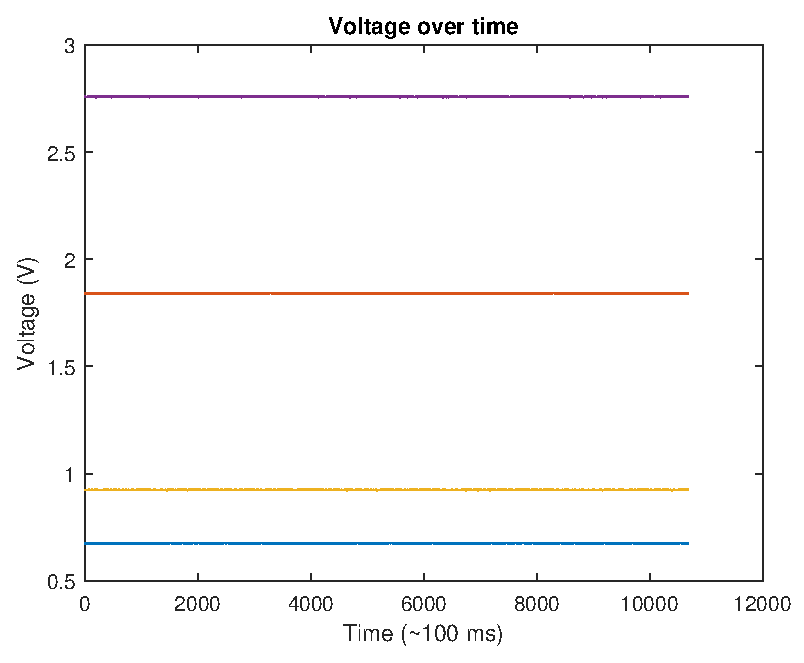
\includegraphics[width=\SchematicWidth]{images/ADC/time-deviation.eps}



% \section{Characterization of the wings}
% \input{\Src/carac/part2/carac-wings.tex}
% [ EDIT :  TO BE DONE ! ]



% \chapter{Mechanical design}
% <<<<<<< HEAD
<<<<<<< HEAD
% This part is 100% on the annexes
=======
test 2
>>>>>>> cd3bfa6 (a test to test if the test was succesfully tested)
=======
test 2
=======
test

\section{Parachute mechanism}
Once launched, the rocket need an safe method to land back on earth. This mean
we need a parachute to be deployed once the rocket has got it's maximal altitude.

But, this parachute need to be safely stored inside on rocket tube while launching,
to prevent any damages !

\subsection{Constraints}
To ensure a correct flight trajectory, we needed to place the parachute (which is a quite
heavy element) near the center of the rocket. This mean there is some stuff above it.

This is an serious constraint, because we can't simply eject the tip of the rocket to
free the parachute, but we need to split the tube in half, while ensuring structural
rigidity of the tube while launching !

\subsection{Solutions}
To circumvent theses constraints, we choose a locking mechanism, based on a rotational lock.

There is two rings, one fixed to the tube, the other fixed to an axle in the middle of the
rocket. Theses two are bound together by four locks, for which a rotating movement of the base
will make them rotate, exposing a solid arm to the outside.

Theses arms are going into slots in the second part of the tube, where they lock themselves into,
maintaining the both part of the tube together.

A final spring has been added in the inferior part of the tube to ensure the top part will be
ejected once the locks are removed.
>>>>>>> b6c5220 (Added a first part of the parachute, waiting for some schematics to explain more in details)
>>>>>>> a5be01c (Conflicts resolved)


\chapter{Electronic design}
Let's talk about the electronic design

First, we're going to dig into the schematic we've done for the physical part
of controller. Thus, we're going to start with a global schematic part, where
we explain the organization of the pages, and then we'll dig a bit deeper into
the differents blocs.

The whole schematic is available at the end of this report, in the annexes
\ref{annex:schematic}.

\section{Power supplies}
Now, let's look a bit deeper on the power supplies, and how they're agenced.
\subsection{Power tree}
To represent the whole power supply organization, we drew a power tree, a schematic that
represent the power supplies.

\input{\Schematics/power-tree.tex}

On this schematic, there two main regulators, that are, in fact buck switching regulators.
But, there's three power sources :
\begin{itemize}[noitemsep]
    \item   Vbus : The 5V that came from the USBC port when the board is plugged on a PC.
    \item   Vbatt : A battery that is charged to power up the MCU and all of the logic
          circuits.
    \item   Vbatt\_pyro : A battery that is charged to power up the servo engines and
          the thruster starter.
\end{itemize}.

As we can see in \ref{fig:power_tree}, we can configure the power supply as we need.
From the three sources, we're able to use a single one by tying both supply together.
And, we can even then supply the whole system with a single USB supply, but at a reduced
voltage. At the opposite, if needed, we can bypass the 5V buck system if we want to
power the servos and the engines with an higher voltage.

Selection is mainly done by jumper, which are big zero ohm resistors.

\subsection{DCDC buck design}
To design theses circuits, we used a reliable tool that may be found online, from
Texas Instruments : \cite{POWERDESIGNER}. We pass them the input conditions, such as
voltage, and the output wanted : voltage and current. The tool output then circuits
than can match the needs, and we need to select one, based on some settings :

\begin{itemize}[noitemsep]
    \item   Space on board
    \item   Cost
    \item   switching frequency
\end{itemize}

Since we didn't require specific criterion on theses aspects, we choose the one that
was the easiest to solder. Then, we import the designed module into the schematic.

\section{Digital part}
For this second part, the digital one we're going to look at the
microcontroller mostly, but also some parts of the whole digital subsystems.
For this part, we mostly got inspired by development kits, such as
\cite{nRF5340DK}. These provide a great example on how to implement some IC on
custom PCBs.

Around the MCU, we added some peripherals IC to fulfill our needs, for examples
:
\begin{itemize}[noitemsep]
    \item An 16 Mb EEPROM, to store flight measurements.
    \item An RGB LED, to indicate status to the user.
\end{itemize}

To ensure the systems are working we sometimes need to modify some elements
from the examples. These changes are always documented in the datsheets of the
components.

Here some examples of things we changed :
\begin{itemize}[noitemsep]
    \item   Change configuration bootstrap to select one mode of the other.
    \item   Configure power supplies needed.
    \item   Configure I2C addresses.
\end{itemize}

\subsection{Pin attribution}
To understand how we assigned to each functions some pins on the MCU, we need
to read the datasheets, mainly the MCU one. It's clearly explained that any
peripheral can be routed to any pins a pin matrix . Nonetheless, there's some
pins that can designed for a specific function. For example, there is two pins
designed for high drain current, where the opposite direction (pull up) is
standard. These pins are designed to handle high speed I2C ! So if we want to
use fast I2C, it's clearly recommended to use them.

The remaining pins were placed arbitrary, because we'll changed that later !
\ref{sec:pin_swap}.

\subsection{Discrete logic}\label{subsec:dis_logic}
On the board, most of the logic is done in software by the MCU. But there's two
hardware functions, related to security features.

These are latching the state of the pin with a DLATCH on the boot of the board,
and an AND gate between the command of the engines and input of the drivers.

This enable us to block the start of engines in hardware rather than by
software only. Thus, if the board is configured as debug mode, it won't be able
to start engines, regardless of the software loaded.

\section{Analog conception}
Now, let's jump into the analog design we've done : 
The analog is quite absent on this board, and we only use it for two purposes :

\begin{itemize}[noitemsep]
    \item   Get the position feedback of the servos.
    \item   Monitor voltages on power rails. 
\end{itemize}

For this part, we're measuring a DC voltage that move between $~0.6 \si{\volt}$
and $~2.4 \si{\volt}$. And, they're moving slowly, it take near one second to get
from one limit to the other ! For the second part, we're measuring a static DC voltage,
just to ensure the battery is present and in it's operating range.

Since the voltages are already in our measurement range, and even more, in the area
where the integrated ADC is quite linear, we don't have a lot of signal conditioning
to do.

We've only designed a filter to remove any high frequency signals that may be picked
by the wires used. Thus, we designed a Sallen-Key active filter, with a 100 Hz cutoff
frequency. This filter is absent from the power supply rail measurements, since they
are located on the PCB, and we can ensure the signal integrity with a proper layout.

The circuit is the following one :
\input{\Schematics/servo-filter.tex}

Using a SPICE simulator, we got this response :
\begin{figure}[!hbt]
    \centering
    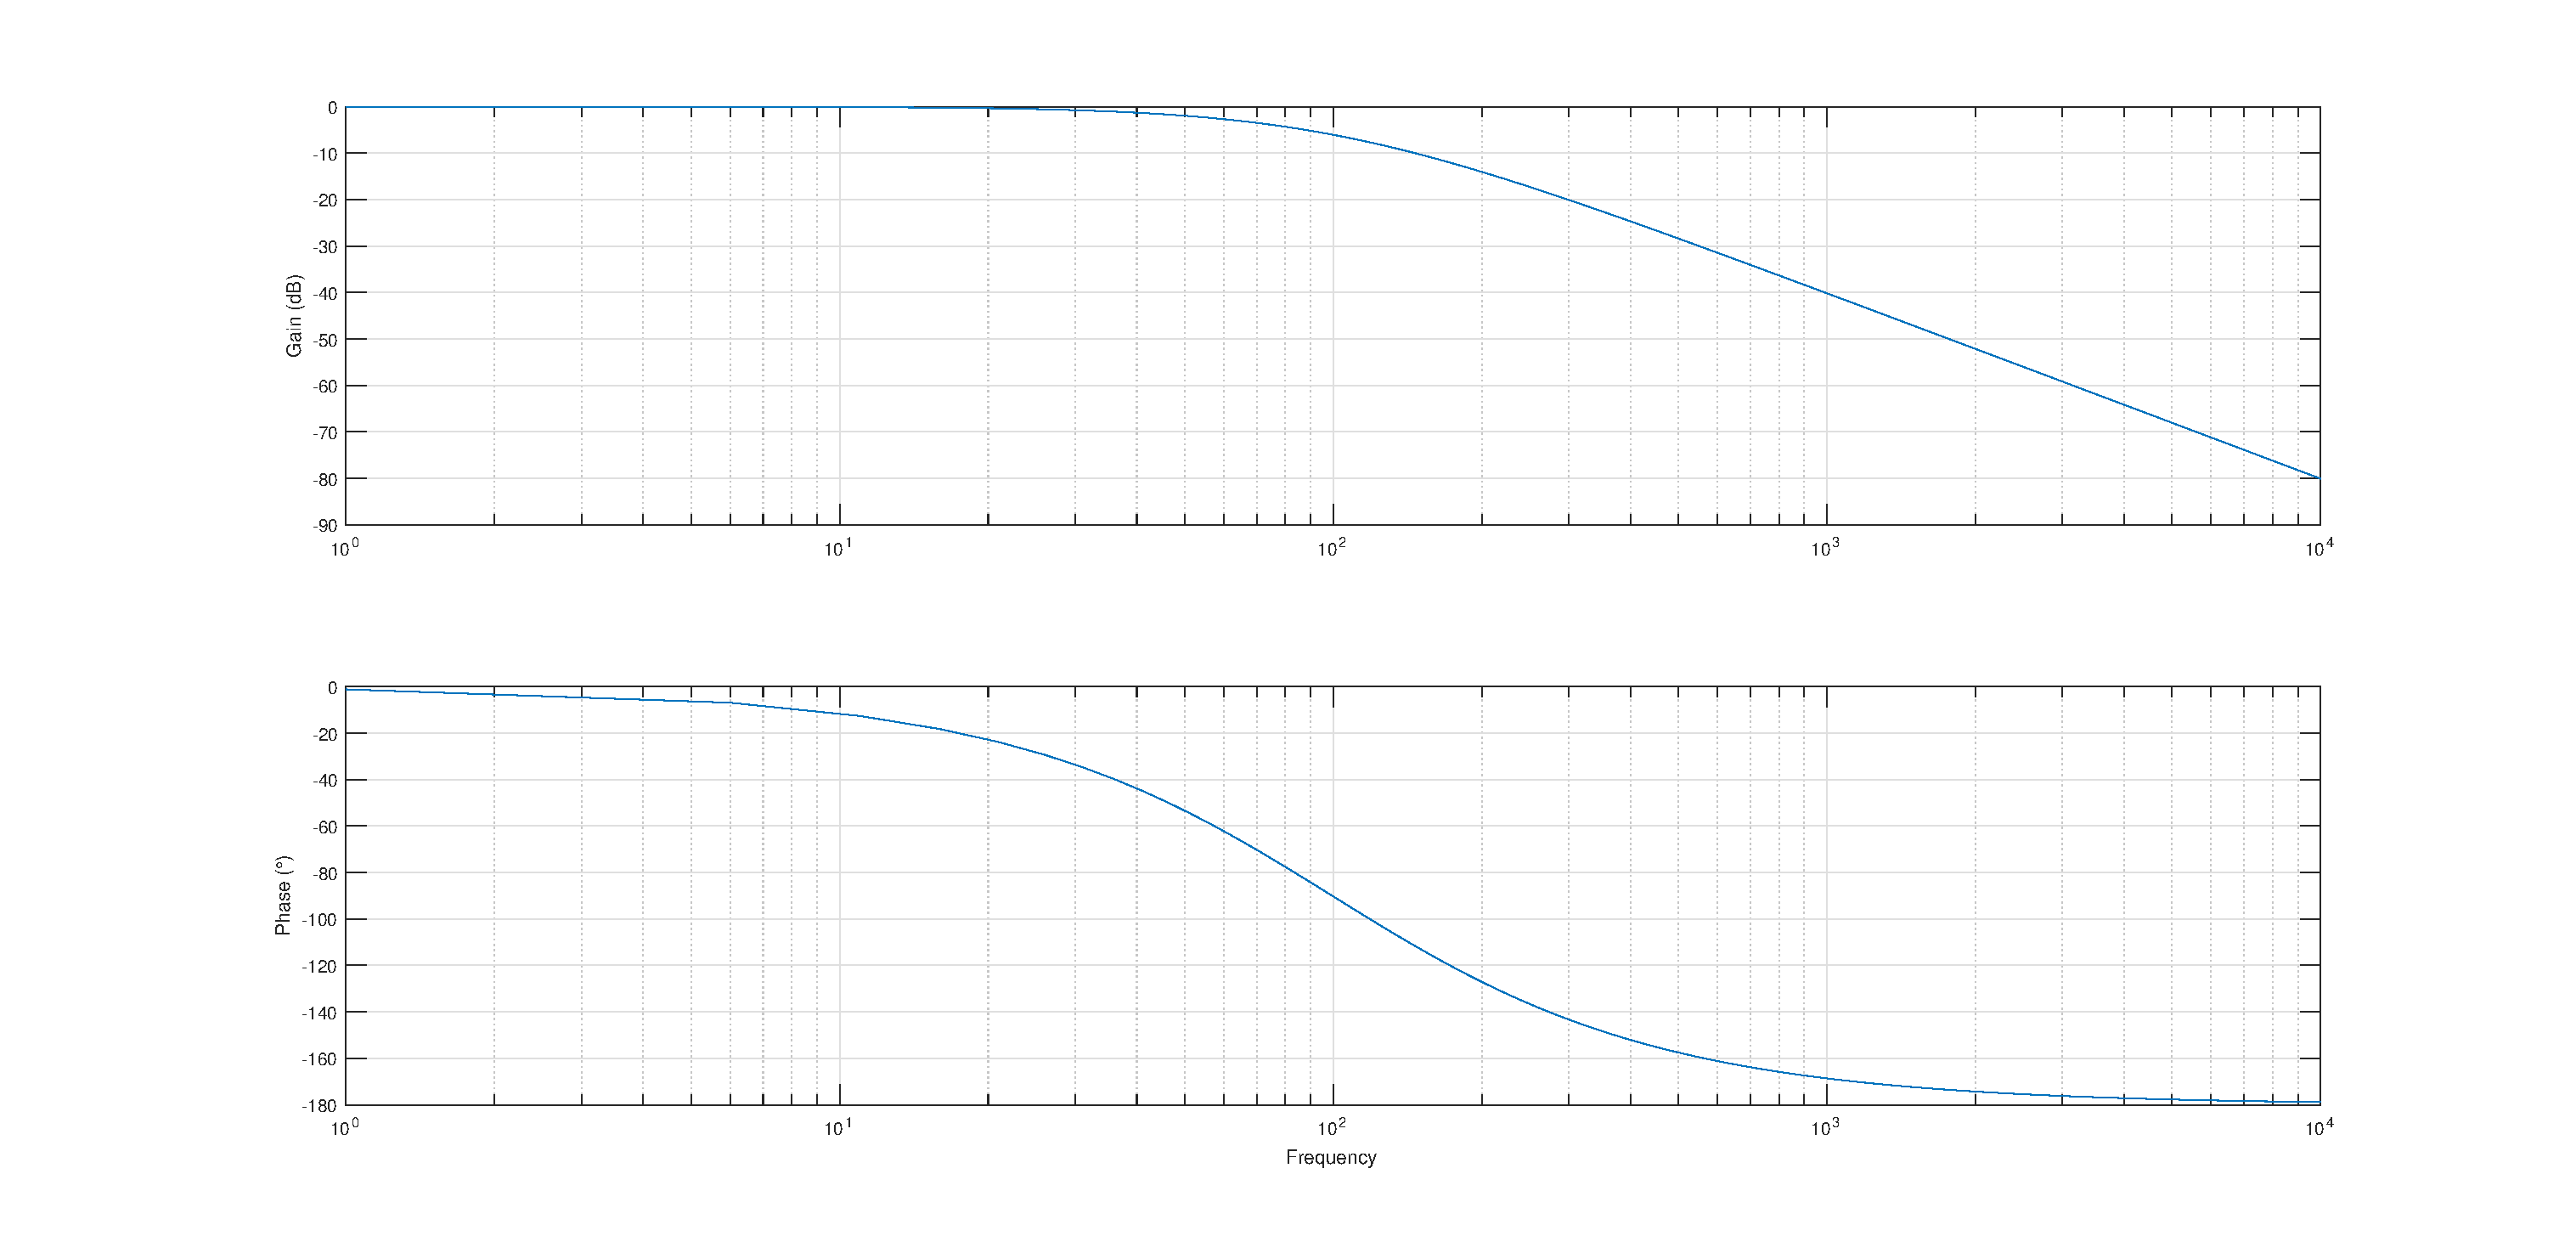
\includegraphics[width=\SchematicWidth]{\Images/Schematic/filter.eps}
    \caption{Bode plot of the filter response}
\end{figure}
\FloatBarrier

The response match our needs, which are quite simple : Remove the potential harmfull noise,
and fast variations that could occur. 

The real circuit on the schematic is based on this one, but with optionnal configurations
jumpers to enable to tune the circuit on board.

This include : 
\begin{itemize}[noitemsep]
    \item   An optionnal voltage divider at the input, to not go above the rail of the OpAmp.
    \item   Optionnals jumpers to bypass the frontend directly to the ADC.
\end{itemize}
\section{Power section}
Now, let's look into the power section of the board. This is this section
responsible to power up the heaviest devices, which can't be powered from a
GPIO.

There's few devices on the board that require specific circuits to be driven :

\begin{itemize}[noitemsep]
    \item   The servomotors (ailerons and parachute).
    \item   The buzzer.
    \item   The engine starters.
\end{itemize}

Each of these elements go it's solution since they're requirements aren't the
same.

\subsection{Servomotors}
These devices are already an integrated solution, we don't directly drive the
servo. So, their power requirements are quite easy to fulfill : We feed them
with 5V, stable voltage.

We only used bulk capacitors near their connectors to ensure that a current
peak is handled it locally.

\subsection{Buzzer}
This second device is a different beast, since we drive it directly. This time,
we placed it directly on the supply, with an NMOS on the low side, to switch on
or off the current on it, and thus make sound, or not.

So, we needed an NMOS transistor to be choosen that can handle some current,
but more importantly : An NMOS that was compatible with our voltage level
available on the output of GPIOs\footnote{ The mosfet we choosed was working,
    the can be optimized : We didn't make sure that is was fully switched at our
    GPIO voltage level, and thats effectively the case : It fully switch at arround
    6V. Thus, the current is limited, which is fine for logic usages but not power
    ones. }.

\subsection{Engine starters}
For these last one, this is where our requirements are the highest : We need a
lot of current, around 2A per engine to start, at a quite high voltage (8-9V).

The power supply for this section is different than the remaining of the board,
for a simple reason : When the engine start, the supply is near the short
circuit. It's voltage will then drop, and it may place others components in
UVLO (UnderVoltage LockOut), where the device stop working.

Here we used ULN2803C drivers IC, made to handle a lot of current with
difficults loads (inductives, high voltage...). These are Darlington BJT
transistors pairs, with each channel done for 500mA. By using four channels in
parallel, we got our current requirements.

But, these IC require arround $ 1 \si{\milli\ampere}$ per input ! Here, that
wasn't an issue since these inputs are controlled by an AND gate
\ref{subsec:dis_logic}. This gate is able to provide more than enough current,
while preserving a low input current, perfect for an MCU or any GPIO.

\section{RF Antennas}
For this second section, we're going to explore some RF design steps that we done on the PCB,
to draw our antennas for the different modules.

This include a $1.55 \si{\giga\hertz}$ for the GPS signals, and a $2.4 \si{\giga\hertz}$
Bluetooth antenna.

For theses antenna, we've found a nice application note from TI \cite{InvertedF} that
show different examples of RF design for $2.4 \si{\giga\hertz}$  Antenna, and \cite{GNSS}
for the $1.55 \si{\giga\hertz}$ one. Since we don't really know how to properly design an
antenna from scratch, we copied theses design into our schematic and PCB while doing a
little bit of MATLAB simulation on the design to ensure the criterions will be matched.


For this section about PCB design, we're going to explain a lot of different
of elements, such as the component placements, the stackup or the layout.

All of theses are going to be explained separately.
\section{Soldering}\label{sec:assembly}
For the last part of the electronic chapter, we're going to talk about
assembly of the board.

The board use complex components, where the packages are BGA, aQFN...
All of the pitch are in the $0.5 \si{\mu\meter}$ range, thus, it's
evident that it won't be possible to solder it with an iron.

To solder theses components, we used a technic based on industrial
processes, which consists of different steps :

\begin{itemize}
    \item   Apply some solder pastes on the pads.
    \item   Place the ICs and passives on their spots.
    \item   Heat the whole board, to make the solder paste melt.
    \item   Let the board cool down.
\end{itemize}

Solder paste is a mix of tin and flux. It's used to create precision
soldering, since it's much easier to get the rigth volume of tin on a
point.

\subsection{Solder paste application}
First, we need to apply solder pastes. The smallest pads are round,
$200 \si{\mu\meter}$ in diameter, and $500 \si{\mu\meter}$ far from the
other.

It's then impossible to place solder paste by hand on this pads.

That's why we used a stencil, that we place over the board, and fix in
place with different tools. Then, we apply some paste on this stencil, and
we spread it on the board with something rigid enough.

This will fill the stencil holes with the right volume of paste, and, if
correctly placed, right over the pads. Once finished, we remove the stencil,
and there shall be right enough paste, we it needs. \footnote{
    Since the paste is about half flux, getting a bit of paste where it shouldn't
    isn't generally an issue. And, with surface tension of melted tin, it will
    generally flow to the contact without issues.
}

\subsection{Placing the SMT}
Once we're satisfied with the paste application, we can start to place components.

This step can be quite long, since it require a lot of application, and concentration.
Hopefully, there is some tools to make it easier, such as Altium assembly assistant,
which will prompt us which reference goes where, and in which orientation.

This make the placement much faster and right.

Once all components are placed, we inspect them. They need to be precisely placed
for all of them\footnote{
    When the board is hot enough, again, the surface tensions of the melted tin will
    tend to place the IC by themselves. Imprecisions can be corrected here, for a
    maximum of half the distance between two pads.
}. In our board, there is 286 of them !

\subsection{Heating}
For the final part, we need to heat the board. There is multiple solutions here,
we can do it on a specific furnace on the FabLab, or, with an hotplate at home.

We tried the second solution for the first board. This plate is going to heat to
$250 \si{\degree}$, heating the whole board in the same time. All of the paste will
melt in the "same" time, and thus all of the solder will be done in one time.

Once finished, we remove the board carrefully of the heating plate, and wait for it
to cool.

All of the process is in photo right below :

\begin{figure}[!hbt]
    \centering
    \begin{minipage}[c]{\SmallSchematicWidth}
        \centering
        \includegraphics[width=\textwidth]{\Images/assembly/assembly_STENCIL.eps}
        \caption*{Stencil placement}
    \end{minipage}%
    \hfill%
    \begin{minipage}[c]{\SmallSchematicWidth}
        \centering
        \includegraphics[width=\textwidth]{\Images/assembly/assembly_PASTE.eps}
        \caption*{Solder paste applied}
    \end{minipage}%
    \hfill%
    \begin{minipage}[c]{\SmallSchematicWidth}
        \centering
        \includegraphics[width=\textwidth]{\Images/assembly/assembly_SMT.eps}
        \caption*{PCB with the SMT placed}
    \end{minipage}%
    \hfill%
    \begin{minipage}[c]{\SmallSchematicWidth}
        \centering
        \includegraphics[width=\textwidth]{\Images/assembly/assembly_HOTPLATE.eps}
        \caption*{PCB on the heating surface}
    \end{minipage}
    \label{img:assembly}
    \caption{assembly process}
\end{figure}
\FloatBarrier

After that whole process, we need to add the few trough hole components, manually.
This is quite fast, since there is not a lot of them.

\chapter{Controller}
Now that we've seen the main physical part of our Rocket as the PCB and the
physics in the appendix. Let's go back to our specifications. Our rocket needs
to support up to 16g of acceleration, we need to acquire the flight data and
finally we need our rocket to be stabilized by 4 ailerons. We'll now talk about
this last part. For a more efficient read about this I'll present you with the
plan that we will follow:

\begin{itemize}
    \item The control theory behind controlling said ailerons and how to integrate those
          equations into simulation software
    \item The application and translation of those simulations to the software.
\end{itemize}

After those three axes we will finally conclude about the controller side of
the rocket.

To finish this introduction, you will see below a schematic of Opale. The
ailerons that we will control are the forwardmost ones. There are not many
reasons apart from the challenge to use such ailerons at the front of a micro
test rocket as the inherent stability of a rocket would be enough for most
rockets of this size. Those ailerons even reduce this stability by firstly
reducing the ratio CG/CP (center of gravity per center of portance, see the
mechanical appendix for more detail). The reason to add such ailerons for our
project is to first and foremost add the challenge and complexity needed for
this project to be worthy of being a TER and secondly in the future, we could
change the software to follow some sort of waypoints in the air for the rocket
to try and follow.

\begin{figure}[!hbt]
    \centering
    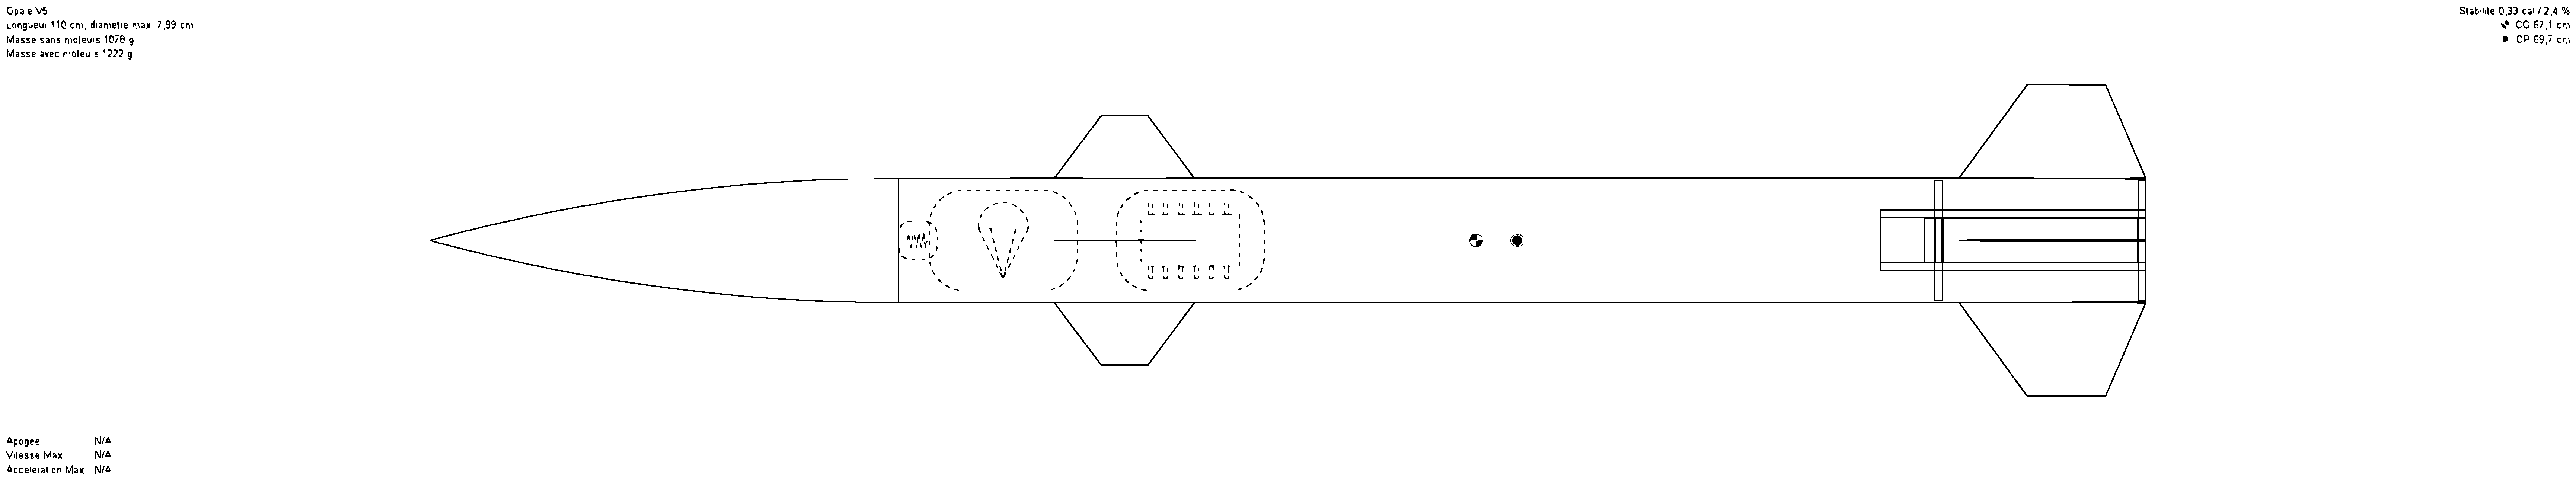
\includegraphics[width=\SchematicWidth]{\Images/mechanical/RocketSchematics.eps}
    \caption{Mechanical schematic of the rocket}
\end{figure}
\FloatBarrier

% Control theory input
\section{The control theory and integration into simulation}
We will now talk about the equations and the control theory behind Opale to be
able to simulate it later and to better comprehend what physical phenomenon
will impact the flight of our rocket to be more precise in the conception of
the body. One thing to be noted is that we will use Euler's equation to
comprehend those

\subsection{Simplified Dynamics of the Rocket with 3 DoF}

\begin{figure}
    \centering
    \resizebox{\SchematicWidth}{!}{%
        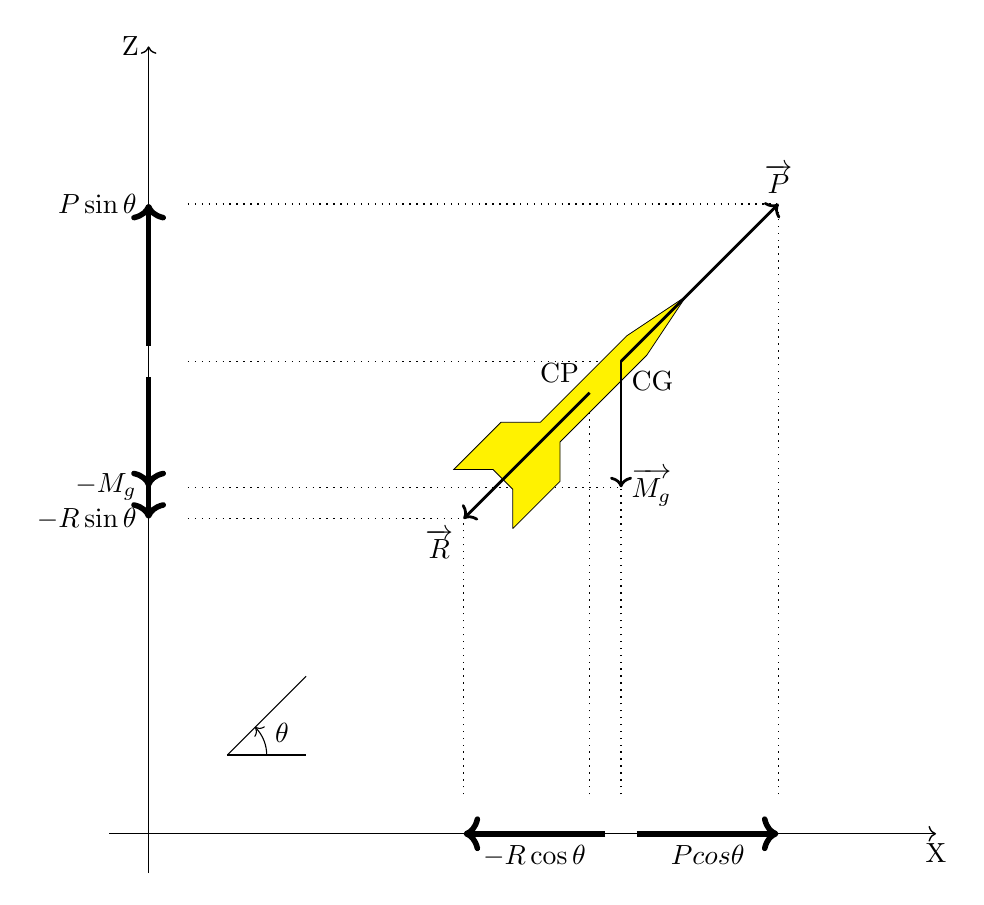
\begin{tikzpicture}
            % adding grid
            \draw [->, line width=0.5pt] (0,-0.5) -- (0,10) node [left] {Z};
            \draw [->, line width=0.5pt] (-0.5,0) -- (10,0) node [below] {X};

            % Adding arrows
            % Horizontals
            \draw[->, line width=2pt] (5.8,0) -- (4,0) node[midway, below]{\(-R\cos{\theta}\)};
            \draw[->, line width=2pt] (6.2,0) -- (8,0) node[midway,below] {\(Pcos{\theta}\)};
            % Vertical
            \draw[->, line width=2pt] (0,5.8) -- (0,4) node[left] {\(-R\sin{\theta}\)};
            \draw[->, line width=2pt] (0,5.8) -- (0,4.4) node[left] {\(-M_g\)};
            \draw[->, line width=2pt] (0,6.2) -- (0,8) node[left] {\(P\sin{\theta}\)};

            % small lines that make the graphe readable
            % Horizontal lines
            \draw [dotted, line width=0.5pt] (0.5,4) -- (4,4);
            \draw [dotted, line width=0.5pt] (0.5,6) -- (6,6);
            \draw [dotted, line width=0.5pt] (0.5,4.4) -- (6, 4.4);
            \draw [dotted, line width=0.5pt] (0.5,8) -- (8,8);
            % Vertical lines
            \draw [dotted, line width=0.5pt] (4,0.5) -- (4,4);
            \draw [dotted, line width=0.5pt] (5.6,0.5) -- (5.6,5.6);
            \draw [dotted, line width=0.5pt] (6,0.5) -- (6,6);
            \draw [dotted, line width=0.5pt] (8,0.5) -- (8,8);

            % Adding the rocket
            \path [draw=black, fill=yellow, line width=0.1mm]
            (4.625,3.875) -- ++(0.6,0.6) -- ++(0,0.5) -- ++(1.1,1.1) --
            ++ (0.5,0.75) -- ++(-0.75,-0.5) -- ++(-1.1,-1.1) --
            ++ (-0.5,0) -- ++(-0.6,-0.6) -- ++(0.5,0) -- ++(0.25,-0.25)
            -- ++(0,-0.5);

            % Adding forces vector
            \draw [->, line width=1pt] (5.6,5.6) node [above left] {CP}-- (4,4) node [below left] {\(\overrightarrow{R}\)};
            \draw [->, line width=1pt] (6,6) -- (8,8) node [above] {\(\overrightarrow{P}\)};
            \draw [->, line width=1pt] (6,6) node [below right] {CG} -- (6,4.4) node [right] {\(\overrightarrow{M_g}\)};

            % Adding angle mark
            \draw (1,1) coordinate(B) -- (2,1) coordinate(A);
            \draw (1,1) -- (2,2) coordinate(C);
            \pic [draw, ->, "$\theta$", angle eccentricity=1.5] {angle = A--B--C};

        \end{tikzpicture}
    }
    \caption{Forces applied to the rocket}\label{img:rocket_forces}
\end{figure}

\FloatBarrier

This rocket can be modeled as a rigid body with 3 degrees of freedom (DoF), but
the control can be focused primarily on pitch and yaw. To follow everything
below we will now see about a 3D case of our rocket this part has been heavily
inspired by the document “Le vol de la Fusée, Stabilité et Trajectographie” by
the CNES \ref{img:rocket_forces}.

If we look a bit into the forces on the rocket in flight we can get the figure
just above and we can take out those 2D equations rather easily:

\begin{minipage}[c]{1\textwidth}
    \centering
    \begin{align*}
        P_x      & = P \times \cos({\theta})   \\
        R_x      & = - R \times \cos({\theta}) \\
        P_z      & = P \times \sin({\theta})   \\
        Weight_Z & = -M \times g               \\
        R_z      & = -R \times \sin ({theta})  \\
    \end{align*}
\end{minipage}
\FloatBarrier

Now that we have our basic equations, we can determine our equations based on
time and in 3D :

\begin{minipage}[c]{1\textwidth}
    \centering
    \begin{align*}
        t_i  & = t_{i-1} + dt \text{: Compute the actual time}                                                                      \\
        m_i  & = m_{i-1} - dm \text{: compute the mass of the roceket as the motor burns fuel}                                      \\
        P_i  & = \text{mean thrust between $t_i$ and $t_{i-1}$}                                                                     \\
        Fr_i & = (P_i - \frac{1}{2}\rho(Z_{i-1}SCx(V_{i-1})V^2_{i-1}) \cos({\text{pitch}_{i-1}})) \text{: Horizontal sum of forces} \\
        Fz_i & = (P_i - \frac{1}{2}\rho(Z_{i-1}SCx(V_{i-1})V^2_{i-1}) \sin({\text{pitch}_{i-1}})) \text{: Vertical sum of forces}   \\
        Gr_i & = \frac{Fr_i}{m_i} \text{: Horizontal acceleration}                                                                  \\
        Gz_i & = \frac{Fz_i}{m_i} \text{: Vertical acceleration}                                                                    \\
        Vr_i & = Vr_{i-1} + Gr_i dt \text{: Horizontal velocity}                                                                    \\
        Vz_i & = Vz_{i-1} + Gz_i dt \text{: Vertical velocity}                                                                      \\
        V_i  & = \sqrt{Vr_i^2 + Vz_i^2} \text{: Total velocity}                                                                     \\
        X_i  & = X_{i-1} + (Vr_i dt + Gr_i \frac{dt^2}{2}) \cos({yaw})\text{: X position}                                           \\
        Y_i  & = Y_{i-1} + (Vr_i dt + Gr_i \frac{dt^2}{2}) \sin({yaw}) \text{: Y position}                                          \\
        Z_i  & = Z_{i-1} + Vzi dt + Gz_i \frac{dt^2}{2} \text{: Z position}                                                         \\
    \end{align*}
\end{minipage}

And, for the pitch :
\begin{itemize}
    \item If the rocket left the launch ramp :
          \begin{itemize}
              \item \begin{gather*}
                        pitch_i  = \arctan{V_{z_i}}{V_{r_i}}
                    \end{gather*}
          \end{itemize}
    \item If the rocket is on the launch ramp
          \begin{itemize}
              \item \begin{align*}
                        Fr_i & = Fr_i - m_i \times g \times cos({pitch_{i-1}}) \times sin({pitch_{i-1}}) \\
                        Fz_i & = Fz_i - m_i \times g \times cos({pitch_{i-1}}) \times cos({pitch_{i-1}}) \\
                    \end{align*}
          \end{itemize}
\end{itemize}

\newpage % Get new page for the flowchart
Those equations can be exported into simulation software like Simulink
following this flow chart :

\begin{figure}[!ht]
    \centering
    \resizebox{0.75\textwidth}{!}{%
        \begin{circuitikz}
            \tikzstyle{every node}=[font=\large]
            \draw [ fill={rgb,255:red,168; green,255; blue,168} ] (12.5,30.75) rectangle  node {\large $\text{Start of calculations :} M_0, V_0, Z_0, \theta_0$} (25,28.25);
            \draw [ fill={rgb,255:red,125; green,190; blue,255} ] (12.5,25.75) rectangle  node {\large $\text{Calculate} M_i$} (25,23.25);
            \draw [ fill={rgb,255:red,125; green,190; blue,255} ] (5,20.75) rectangle  node {\large $\text{Calculate} \gamma X_i (\text{Depends} n R_{i-1} and cos \theta_{i-1})$} (17.5,18.25);
            \draw [ fill={rgb,255:red,125; green,190; blue,255} ] (20,20.75) rectangle  node {\large $\text{Calculate} \gamma Y_i (\text{Depends} n R_{i-1} and sin \theta_{i-1})$} (32.5,18.25);
            \draw [ fill={rgb,255:red,125; green,190; blue,255} ] (5,15.75) rectangle  node {\large $\text{Calculate} V\gamma_i (\text{Depends on} Vx and \gamma_i)$} (17.5,13.25);
            \draw [ fill={rgb,255:red,125; green,190; blue,255} ] (20,15.75) rectangle  node {\large $\text{Calculate} Vz_i (\text{Depends on} Vz_{i-1} and \gamma_i )$} (32.5,13.25);
            \draw [ fill={rgb,255:red,125; green,190; blue,255} ] (5,10.75) rectangle  node {\large $\text{Calculate} the x_i (\text{Depends on} X_{i-1} and \gamma X_i)$} (17.5,8.25);
            \draw [ fill={rgb,255:red,125; green,190; blue,255} ] (20,10.75) rectangle  node {\large $\text{Calculate} Z_i (\text{Depends on} Z_{i-1} and \gamma Z_i)$} (32.5,8.25);
            \draw [ fill={rgb,255:red,125; green,190; blue,255} ] (12.5,5.75) rectangle  node {\large $\text{Calculate} V_i$} (25,3.25);
            \draw [ fill={rgb,255:red,125; green,190; blue,255} ] (12.5,0.75) rectangle  node {\large $\text{Calculate} R_i$} (25,-1.75);
            \draw [ fill={rgb,255:red,125; green,190; blue,255} ] (12.5,-4.25) rectangle  node {\large $\text{Calculate} \theta_i$} (25,-6.75);
            \draw [ fill={rgb,255:red,251; green,223; blue,249} ] (12.5,-9.25) rectangle  node {\large Does the rocket has landed ?} (25,-11.75);
            \draw [ fill={rgb,255:red,255; green,128; blue,128} ] (12.5,-14.25) rectangle  node {\large End of calculations} (25,-16.75);
            \draw [->, >=Stealth] (18.75,28.25) -- (18.75,25.75);
            \draw [->, >=Stealth] (11.25,22) -- (11.25,20.75);
            \draw [->, >=Stealth] (26.25,22) -- (26.25,20.75);
            \draw [->, >=Stealth] (11.25,18.25) -- (11.25,15.75);
            \draw [->, >=Stealth] (26.25,18.25) -- (26.25,15.75);
            \draw [->, >=Stealth] (11.25,13.25) -- (11.25,10.75);
            \draw [->, >=Stealth] (26.25,13.25) -- (26.25,10.75);
            \draw [->, >=Stealth] (18.75,7) -- (18.75,5.75);
            \draw [->, >=Stealth] (18.75,3.25) -- (18.75,0.75);
            \draw [->, >=Stealth] (18.75,-1.75) -- (18.75,-4.25);
            \draw [short] (11.25,22) -- (26.25,22);
            \draw [short] (18.75,23.25) -- (18.75,22);
            \draw [short] (11.25,8.25) -- (11.25,7);
            \draw [short] (11.25,7) -- (26.25,7);
            \draw [short] (26.25,8.25) -- (26.25,7);
            \draw [->, >=Stealth] (18.75,-6.75) -- (18.75,-9.25);
            \draw [->, >=Stealth] (18.75,-11.75) -- (18.75,-14.25)node[pos=0.5, fill=white]{YES};
            \draw [short] (12.5,-10.5) -- (2.5,-10.5)node[pos=0.5, fill=white]{NO};
            \draw [short] (2.5,-10.5) -- (2.5,24.5);
            \draw [->, >=Stealth] (2.5,24.5) -- (12.5,24.5);
        \end{circuitikz}
    }%
    \caption{Algorithm used to simulate the rocket trajectory.}
    \label{fig:my_label}
\end{figure}
\subsection{The rotational equation to make our model with 6DoF}

We now have our equations to compute the position and its derivatives over
time. The thing is those equations are only for a rigid body with only 3 DoF
and without any ailerons added to them. To be able to have our 6 DoF and to be
able to input our ailerons into this simulation we need to refer to Euler's
equation of rotational dynamics as well as the standard aerodynamic lift
equations:

For a rigid body\footnote{rigid body is symmetrical and the axes are aligned
    with the frame} with a diagonal inertia tensor:
\begin{gather*}
    \begin{cases}
        r_x = I_x \dot{\omega}_x - (I_y - I_z)\omega_y \omega_z \\
        r_y = I_y \dot{\omega}_y - (I_z - I_x)\omega_z \omega_x \\
        r_z = I_z \dot{\omega}_z - (I_x - I_y)\omega_x \omega_y
    \end{cases}
\end{gather*}

with $r$ the net torque, $I_\omega$ the angulor momentum, $I$ the inertia
tensor and $\omega$ is the angular velocity.

We can assume that the rocket is symmetrical so $I_x=I_y$ and we could
calculate the $I_z$ but we would see that if the rocket is long but slim it
tends to be small. We consider as well that the pitch and yaw are coupled but
the roll isn't coupled with the rest.

We now find thoses equations :
\begin{gather*}
    \begin{cases}
        r_x = I_x \dot{\omega}_x - (I_x - I_z)\omega_y \omega_z \\
        r_y = I_x \dot{\omega}_y - (I_z - I_x)\omega_z \omega_x \\
        r_z = I_z \dot{\omega}_z
    \end{cases}
\end{gather*}

We can integrate those equations into the simulation like this:

\begin{align*}
    \dot{\omega}_x & = \frac{1}{I_x}(r_x + (I_x - I_z)\omega_y \omega_z) \\
    \dot{\omega}_y & = \frac{1}{I_x}(r_y + (I_z - I_x)\omega_z \omega_x) \\
    \dot{\omega}_z & = \frac{I_z}r_z                                     \\
\end{align*}

And we can integrate them over time to get orientation rates like this :

\begin{gather*}
    \dot{\omega}_i(t + dt) = \omega_i(t) + \dot{\omega}_i dt
\end{gather*}

Because we use Euler's equations, we encounter a problem known as the gimbal
lock. This happens as two rotation axes become aligned. Because we are in a 3D
space instead of a 4D space like for quaternions, we can't differentiate
between those two axes and so we lose a DoF as long as those axes are merged.

% Aerodynamics
\subsection{Aerodynamics equations for the ailerons}

Now for the ailerons we choosed the NACA-0009 at 9\% fill design for ailerons,
which is used for most control surfaces of this size because it grants a
sufficient lift coefficient as well as a good linear lift region. It grants
about 14 to 16 degrees before our aileron stalls. We assume that this is with a
relatively high number of Reynolds which we have a chord of 9 cm. We can see
this thanks to this equation :

\begin{gather*}
    R_e = \frac{\rho V c}{\mu}
\end{gather*}

with $c$ the chord lenght and $V$ the airflow on the ailerons.

So, with our rocket going at max at $130 \si{\meter\per\second}$ and with a
chord length of $9 \si{\centi\meter}$ we have $8.05 \times 10^{-5} Re$ which is
considered high ($10^5 \text{ to } 10^6 \space Re$ is considered high in
aviation) we can also calculate that our ailerons would have a flow separation
between each side of the ailerons at approximately $10 \si{\degree}$ to $12
    \si{\degree}$ of angle of attack (AoA) which would render our control of the
flow non-linear. So, with this in mind we can limit our AoA at 10° at most in
the embedded code as well as in the simulation.

\begin{figure}[!hbt]
    \centering
    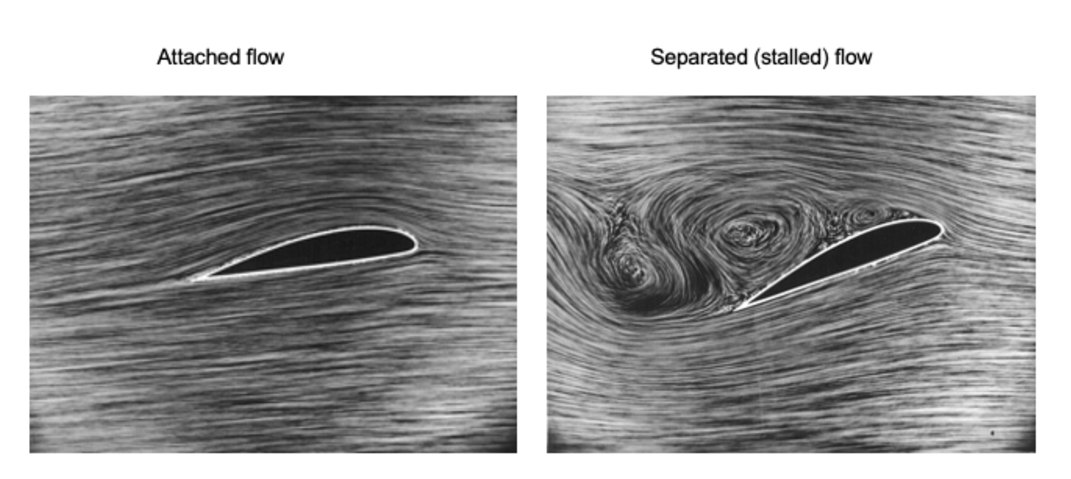
\includegraphics[width=\SchematicWidth]{\Images/mechanical/AirfloilStall.eps}
    \caption{Mechanical schematic of the rocket}
\end{figure}
\FloatBarrier

Now to be able to simulate those ailerons we need to be able to calculate the
torque generated by each aileron to add into the equation of rotation we saw
just above. For each aileron we can determine their impact on the total torque
generated with :

\begin{align*}
    F_L  & = \frac{1}{2} \rho V^2 S C_L (\delta)                     \\
    \tau & = r * F_L                                                 \\
         & = r ( \frac{1}{2} \rho V^2 S C_{L \delta} \times \delta)  \\
         & = \frac{1.006 \times 160 \times 0.09}{1.8 \times 10^{-5}} \\
         & = 8.05 \times 10^{-5}                                     \\
\end{align*}

We can say that :

\begin{gather*}
    K_\tau = \frac{1}{2} \rho V^2 S C_{L \delta} r
\end{gather*}

And thus:

\begin{gather*}
    \tau = K_\tau \times \delta
\end{gather*}

With $V$ the velocity, $S$ the surface $C_{L \delta}$ the derivative of the
lift coefficient, $F_L$ the lift force, $\tau$ the torque, $K_\tau$ the control
effectiveness coefficient, $\delta$ the AoA and r the moment arm which is the
distance between the $CL$ and the $CM$ of the rocket.

To integrate those equations into the simulation we only must determine the
angles of our ailerons over time and input it in the previous equations :

\begin{gather*}
    \tau_i = \frac{1}{2} \rho V^2 S C_{L \delta} r \times \delta_i
\end{gather*}

Our $\delta_i$ will be computed through the output of our simulated PID which
we will see just below this.

With this we can now create our own simulation. We just need to add a few
gaussian noise generators to our system to test our resistance to noise, a
thrust curve to input our thruster in there and a delay between the controller
and the actuators to test even further our model. Which can resemble this:

\begin{figure}[!hbt]
    \centering
    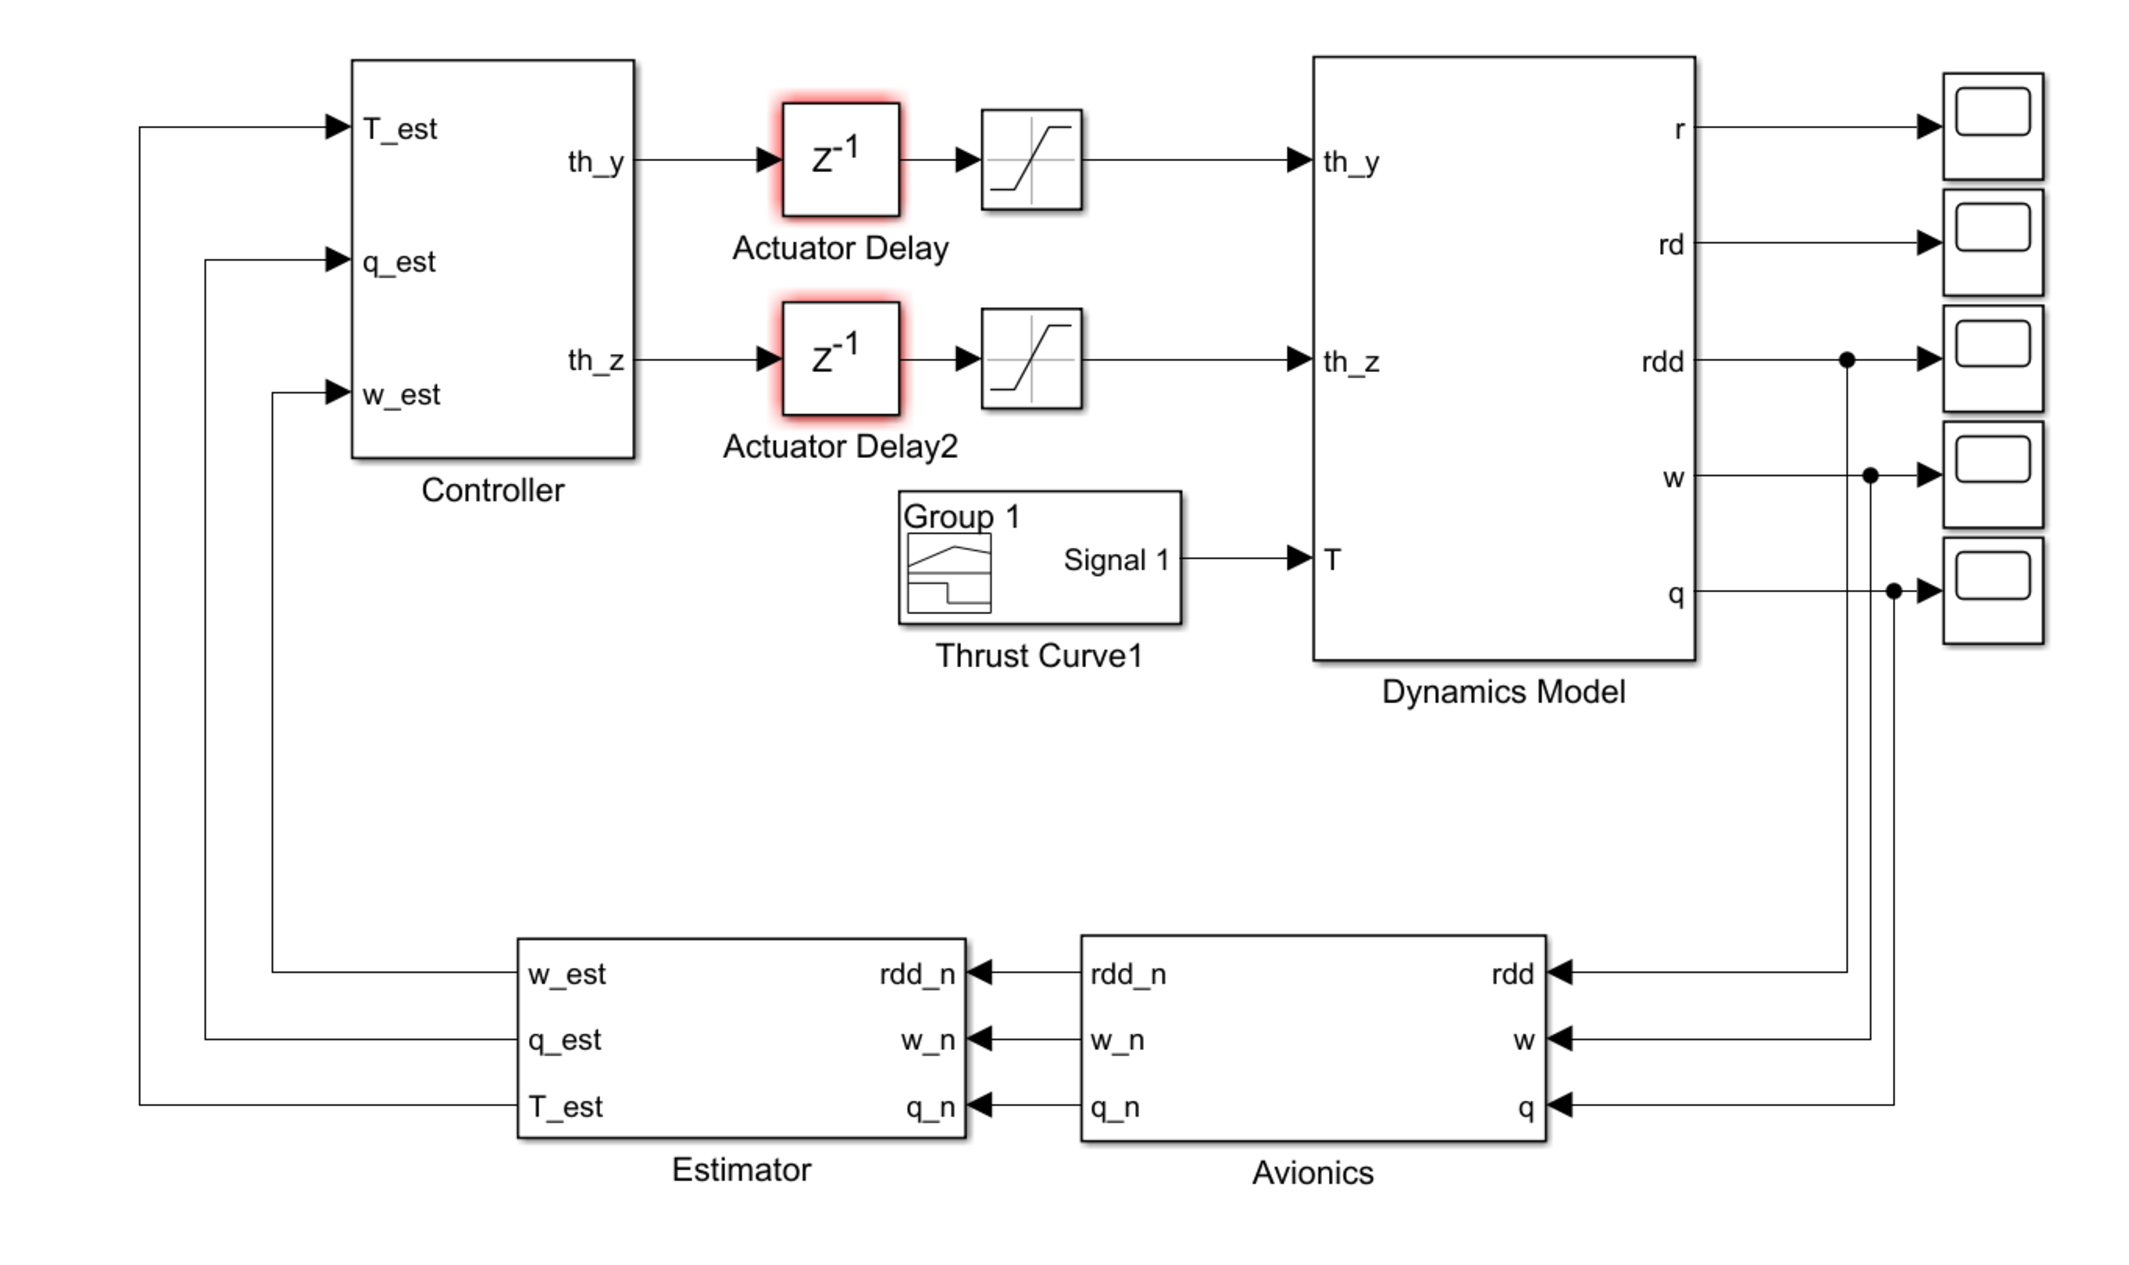
\includegraphics[width=\SchematicWidth]{\Images/rocket_sim/simulink.eps}
    \caption{Simulink model we used}
\end{figure}
\FloatBarrier

To complete our simulation and to be able to compute the angles of every
aileron we need to have some sort of controller. In our case, we will use a PID
controller as it is the controller I am most comfortable with and the one I
understand the most. We create in fact 3 different PID for each axis:

\begin{gather*}
    \delta_{CMD}(t) = K_P e(t) + K_D \frac{de(t)}{dt} + K_I \int e(t) dt
\end{gather*}

with $e(t)$ the error between the command and the feedback.

After combining each PID we have :

\begin{gather*}
    \overrightarrow{\delta} = M_{control} *
    \begin{bmatrix}
        \delta_P \\
        \delta_Y \\
        \delta_R
    \end{bmatrix}
\end{gather*}

With which we can determine a control matrix to find the effect of each aileron
on a specific axis for example what we have as a control matrix is :

\begin{gather*}
    M_{control} =
    \begin{bmatrix}
        +1 & +1 & +1 \\
        +1 & -1 & -1 \\
        -1 & -1 & +1 \\
        -1 & +1 & -1 \\
    \end{bmatrix}
\end{gather*}

This matrix controls which ailerons move in which direction.

\begin{figure}[!hbt]
    \centering
    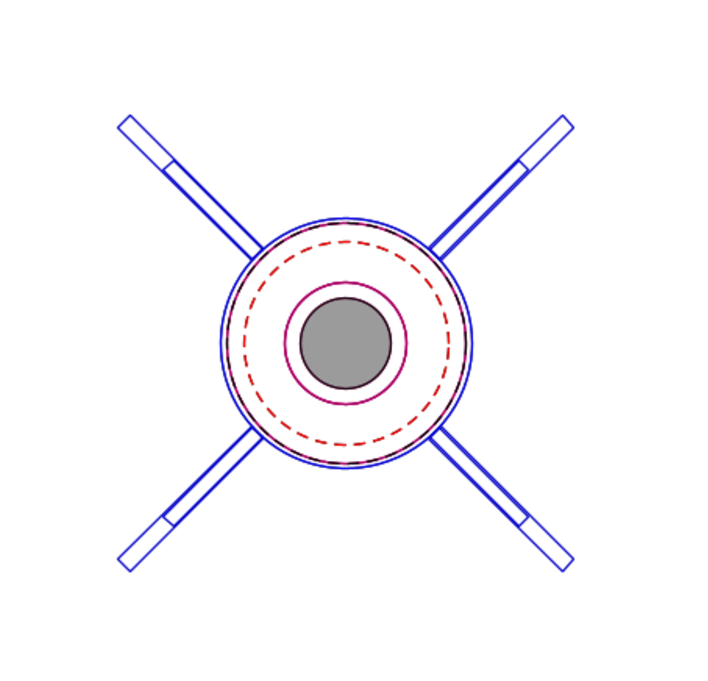
\includegraphics[width=\SchematicWidth]{\Images/mechanical/AileronsPosition.eps}
    \caption{Simulink model we used}
\end{figure}
\FloatBarrier


\chapter{Programmation}
\paragraph{}
For this part, let's talk about a whole different beast : The software. This
correspond to all of the code executed on the microcontroller to command all of
the actions done, from the control of the rocket trajectory to the log of the
temperature !

\paragraph{}
This is a very complex topic, that could be the subject of a whole report, so
we're forced to reduce some part of it. Nonetheless, we'll go through all of
the main subjects. First, we'll talk about the configuration of the different
functions by exploring the different devicetree files. In a second time, we'll
go trough the fundamentals of Zephyr RTOS, which was used to schedule main
tasks and handle the scheduling and context switching for ourselves. Then,
we'll start to ramp up into the different abstraction layers used, from the
drivers to the threads. To conlude this chapter, we're going to show the global
software architecture we used over the project.

% Including all of the files
% Device trees
\section{Configuration using devicetrees}
Since we're using a microcontroller that is widely available, most of the work with 
devicetrees has already been done by the manufacturer.

Thus, we don't need to care about memory, cpus, or other internals details of the
peripherals. We only edit properties that are related to our needs, which include
peripherals or other ICs.

All of the structure was automatically generated by a tool provided by the manufacturer, 
that create an empty structure with everything needed to ensure the boot of the controller.

\paragraph{}
To make the structure cleaner, we've used a lot of overlays, because it's much easier
to debug and find the right property when needed.

\subsection{Main overlays}
Thus, the generated file has only a new line : the one needed to include the main overlay file.

This file look like this :

\inputminted[linenos, firstline=16, lastline=44]{devicetree}{\DeviceTree/topaze-pinctrl.dtsi}

This file is not a properly formed overlay, since it does indeed overlay nothing. But it make our
job easier by grouping all of the sub includes into a single file. Then, we can modify them for
debugging purposes.

We'll quickly move to another file that show a real overlay file, such as the PWM and I2C configuration.

\subsection{Peripherals overlays}
\subsubsection{PWM configuration}
Then, let's open a file like the PWM configuration to explore more in details what an overlay is.
For any overlay file, we used four main blocks\footnote{
    The number of block may vary depending on each architecture and software decision.
}, which are

\begin{itemize}
    \item Global peripheral configuration
    \item Pin configuration
    \item Advanced peripheral configuration
    \item Aliases
\end{itemize}

\paragraph{Global peripheral configuration} ~\\
First, we need to configure globally the peripheral.
\inputminted[linenos, firstline=17, lastline=21]{devicetree}{\DeviceTree/topaze-pwm-servo.dtsi}

Here, we're simply enabling the peripheral by setting it's status property to "okay". Then, we're 
passing a reference to a pinctrl configuration, charged to define the pins. \footnote{
    The default name is mandatory, and is used by the RTOS to know what to do with theses pins once 
    placed in low power modes. We're not using them here.
}

\paragraph{Pin configuration} ~\\
Then, right after, we're configuring the said pins. We pass a group of pins that are defined by a 
macro, that return the pin number according input like the port, the pin, and some description.

\inputminted[linenos, firstline=24, lastline=33]{devicetree}{\DeviceTree/topaze-pwm-servo.dtsi}

As previously said, we're not using low power modes so we don't need them in our project. If they 
were defined, we would see here two group of pins, one for each mode.

\paragraph{Advanced peripheral configuration} ~\\
Now, the main configuration part. That's where we configure most of the behavior of the PWM peripheral.

\paragraph{}
Before entering into the main details, we need to explain something : We created a node named "wings" here, 
that is compatible with pwm-wings. This is a custom wrote specification for our needs that wait for 
\begin{itemize}
    \item A pwm array with exactly four pwm channels
    \item A pwm period
    \item Some boundaries about the duty cycle (expressed in time domain)
\end{itemize}

\inputminted[linenos, firstline=52, lastline=66]{devicetree}{\DeviceTree/topaze-pwm-servo.dtsi}

Thus, we find here our custom node with our four servo-engines defined, and some settings.
Not all settings are used by the PWM peripheral to configure itself, but by the software that 
import them as constants.\footnote{
    For example, min-pulse and max-pulse are used by the software to compute the required 
    pulse for a defined angle.
}

\paragraph{Aliases} ~\\
Then, to conclude on this file, we define some aliases. Theses enabled the fetching of a node by quoting
it's name rather than it's location. 

\inputminted[linenos, firstline=69, lastline=74]{devicetree}{\DeviceTree/topaze-pwm-servo.dtsi}

\subsubsection{I2C configuration}
Then, in the same manner we configured the I2C \footnote{
    And a lot of other peripherals !
}. The file expose the same structure, as any overlay in the project. 

\inputminted[linenos, firstline=36, lastline=61]{devicetree}{\DeviceTree/topaze-I2C.dtsi}

The main difference with the previous file is the presence of multiple nodes here, once for each I2C sensor.
Each device can has some properties, such a compatible, status and reg properties. The last one, reg, 
correspond to it's address on the bus ! Thus, we don't care about such details on the software, we communicate
with a sensor, not a peripheral on some address.

\subsection{Final words}
To conclude this part, let's resume a bit the devicetree files. Theses are used for hardware related configuration, 
and expose some options that may be used to directly configure the registers of an IC, or be exposed to a C or C++ 
as constants for more advanced usage. They're used by the underlying OS on the MCU while the pre-kernel boot.

Theses files are complex to write, but can be used to configure precisely the differents hardware while reducing 
user errors.


% Drivers
\section{Drivers}
Next in the hierarchy, we found the drivers. This codes are used to prevent from the
user to perform low-level IO, which are error prones.

\paragraph{}
All of them are written by the manufacturer or the chip, in our case, Nordic
Semiconductors.
Theses contain mostly definitions about structures passed to the driver to
configure an element, of function that we may call.

\subsection{Calling the driver}
Theses drivers can be called by two distinct ways :
\begin{itemize}
    \item From bare-metal code
    \item From Zephyr RTOS drivers, who redirect calls to the bare-metal code
\end{itemize}

The second method is the safest, in the manner that the RTOS handle the request for us,
but, to ensure compatibility with a lot of chips, it can't provide exact same options as
the bare metal driver.

That's why we used both, mostly the Zephyr one were we could.

\subsection{Driver usage}
\subsubsection{Bare metal}
To give an example of the driver beeing used, there is the initialization code the ADC module

\inputminted[linenos, firstline=103, lastline=112]{cpp}{\Code/peripherals/saadc/saadc.cpp}

This code is responsible for the configuration of some advanced behaviors of the ADC peripheral,
such as setting it's resolution, callback function and so.
Calls are here quite long, because of the different structs that need to be configured, defined,
and applied for each aspect.

\subsubsection{Zephyr}

On the other hand, here the example for the Zephyr driver being called.
This is much simpler, because we're here calling the Zephyr Driver that handle a lot of the work
for us, based on the devicetree !

\inputminted[linenos, firstline=100, lastline=102]{cpp}{\Code/devices/servo/servo.cpp}

We just need to care about the pulse length we want to set. All the other parameters were defined
when the kernel was booting.







\section{Device drivers}
Next, let's ramp a bit higher in the software structure. Now that we have drivers for
most simple peripherals, we'll need drivers for devices, to handle all of the specific 
protocols for us.

Thus, when we need to read a temperature, we don't want to write to a register, wait for 
some time, and then read. We want to call a function that return us the temperature.

That's the exact job for a device-driver. 
It format requests, use the peripherals drivers to handle the IO, and then make some 
calculations to return us a precise value in any cases.

These kind of drivers can be sourced from the manufacturer, but some need to be wrote by
hand. Others need to be modified to be compatible with our software decisions. Some 
other only provide standard libraries for the drivers, and let the user develop they're
own drivers.

\subsection{Manufacturer sourced drivers}
In the first case, which is the preferred option, the work needed is generally small.
For example, the driver for the IMU was entirely wrote by Bosch, which require us to 
write only the communication functions !

This look like :
\inputminted[linenos, firstline=19471, lastline=19515]{cpp}{\Code/drivers/bno055/bno055.cpp}

And, that's done for the driver !

\subsection{Libraries based drivers}
In this second case, the manufacturer only provided some standard libraries to be used.
An lot of work was needed to ensure this driver is correctly working. 

In the previous code section, the manufacturer provided a write and read functions to be
called. It only required us to fill them.

\inputminted[linenos, firstline=292, lastline=330]{cpp}{\Code/drivers/teseo/teseo.cpp}

Hopefully, manufacturer provided us some functions to check if a command was well 
formed, to match the checksum, as well as some parsers to identify the different 
elements. 

This save us a lot of time compared to writting the full driver.

In this example of code, the manufacturer provided the GNSS\_PARSER\_CheckSanity functions
and other return values codes.

We only needed to implement the IO.

\subsection{Hand written drivers}
Even if theses drivers are quite complex to write, they're generally reserved to much 
smaller chips, which make the develop quite straightforward. 
For example, the only driver we needed to develop like that was for the temperature
sensor.

\inputminted[linenos, firstline=119, lastline=158]{cpp}{\Code/drivers/ms5611/MS5611.cpp}

This driver include all of the calculations needed for temperature corrections
needed to match the precision. Theses are indeed affected by temperature, 
or just measure range. The sensor isn't linear at all over the plage, but per 
segments.

Here, all of the code was hand written because nothing, except documentation was provided.


\subsection{Final words}
To conclude this part on drivers, we can resume them as a fundamental brick of the software, 
that handle all of the device specific requirements.
This part part is generally where the errors are, because they're difficult to test entirely.

% Gloval architecute
\section{Architecture}
For this final section on the software architecture, let's talk about the top of the pyramid.
Now, we have a fully configured chip, devices drivers, and an RTOS ready to handle task.

We just need to create the differents elements to communicate, and connect them together.

...


% Set page number in uppercase roman (I, II, III)
\chapter*{Conclusion}
\pagenumbering{Roman}

\addcontentsline{toc}{chapter}{Conclusion}
\paragraph{}



\addcontentsline{toc}{chapter}{Bibliography}
\printbibliography

\newpage

% Set page number in Alph (A, B, C ...) for annexes
\pagenumbering{Alph}
\appendix

\input{\Src/components/components-annexes.tex}
\input{\Src/carac/carac-annexes.tex}
\chapter{Mechanical Design}\label{annex:mechanical}
In this appendix, we will talk about our different mechanical choices about our micro-rocket Opale.
First things first, to at least be able to start working on our rocket we choose our specifications somewhat arbitrarily. And to choose them we used an app called Open Rocket which is an open-source model rocket simulator.

\section{Tube selection}
At the very beginning, we simply chose a body with a plastic tube called 'Quantum'.
I have one of these tubes at home which is approximately 1.2 m tall. Since we had
to choose a height for the rocket, we decided to make it approximately 1 m tall,
including the motor, ailerons and nose.

\begin{figure}[!hbt]
    \centering
    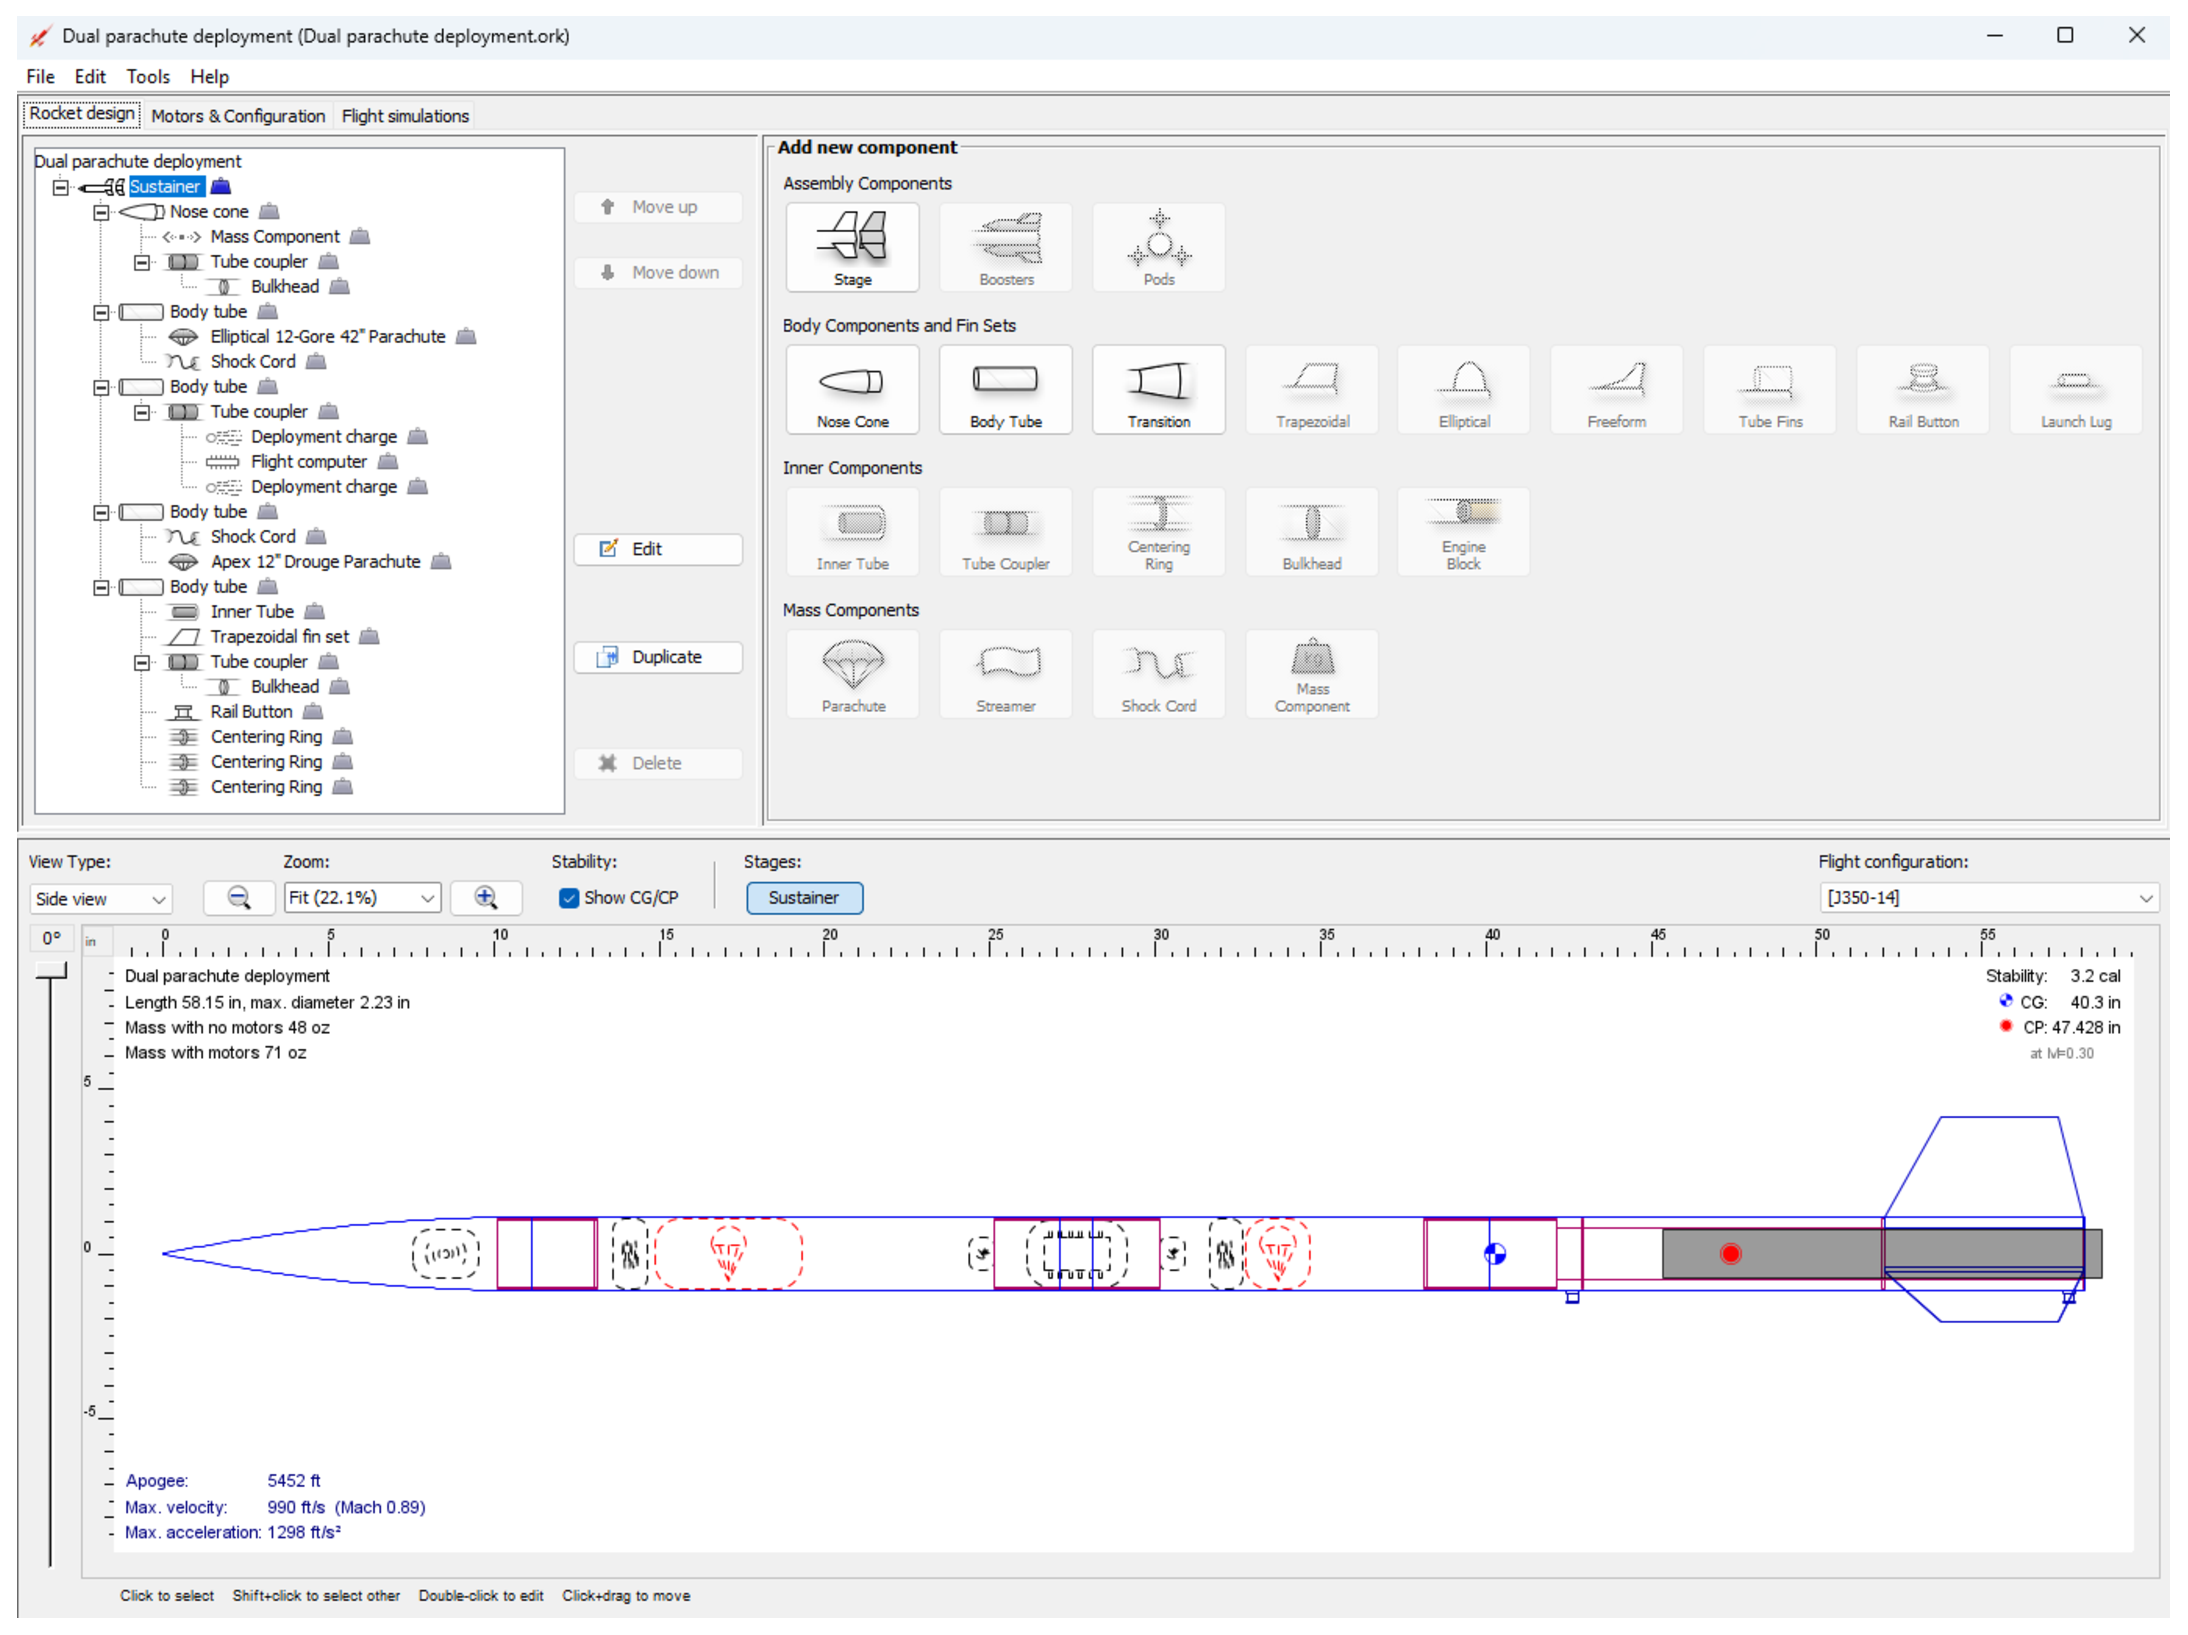
\includegraphics[width=\SchematicWidth]{\Images/mechanical/OpenRocket.eps}
    \caption{Screenshot of the tool used design and simulate rockets.}
\end{figure}
\FloatBarrier

\paragraph{}
One of the most important aspects of building a model rocket is the CG/CL ratio,
and this is something we had to consider. This ratio represents the division between
the position of the centre of gravity and the centre of lift. It represents the
rocket's inherent stability. Our centre of gravity needs to be in front of the
centre of lift, following the axis of our rocket body. The ratio needs to be at
least 1 for the rocket to be stable without an active stabilisation system.

\paragraph{}
For this project, we challenged ourselves by choosing to add active stabilisation
to our rocket in the form of ailerons for control surfaces. We positioned them at
the front of the rocket to maintain the stabilisation provided by the rear ailerons
while retaining control over the rocket's direction. Due to the complexity of the
equations, we chose to ignore the turbulence caused by the front ailerons on the
rear ailerons.

\paragraph{}
One issue arising from the front control ailerons is that they reduce the CG/CL
ratio, as we have added lift to the front of the rocket, thus advancing the CL.
This gave us a ratio of about 0.5, which is considered unstable. This would be
undesirable for a normal rocket, but because our rocket is actively stabilised,
we can afford this kind of trade-off.
We used Open Rocket to design the nose cone of the rocket, which gave us an idea
of the different types of nose cone used in model rockets. We chose the simplest
option: an ellipsoidal cone.

\paragraph{}
To keep things simple, we will 3D print the nose cone and use acetone to smooth
the outer part. We did the same for all eight ailerons and the four control and
static surfaces.

\paragraph{}
Another problem of our rocket is to hold the rocket motor. Our rocket is mostly
composed of plastic and so it will melt at the contact of the motor. We choose
cork which is very poor conductor of heat to hold our motor.

Every part we talked about is to be built in the near future and assembled.

\section{Parachute mechanism}
Once launched, the rocket need an safe method to land back on earth. This mean
we need a parachute to be deployed once the rocket has got it's maximal altitude.

But, this parachute need to be safely stored inside on rocket tube while launching,
to prevent any damages !

\subsection{Constraints}
To ensure a correct flight trajectory, we needed to place the parachute (which is a quite
heavy element) near the center of the rocket. This mean there is some stuff above it.

This is an serious constraint, because we can't simply eject the tip of the rocket to
free the parachute, but we need to split the tube in half, while ensuring structural
rigidity of the tube while launching !

\subsection{Solutions}
To circumvent theses constraints, we choose a locking mechanism, based on a rotational lock.

There is two rings, one fixed to the tube, the other fixed to an axle in the middle of the
rocket. Theses two are bound together by four locks, for which a rotating movement of the base
will make them rotate, exposing a solid arm to the outside.

Theses arms are going into slots in the second part of the tube, where they lock themselves into,
maintaining the both part of the tube together.

A final spring has been added in the inferior part of the tube to ensure the top part will be
ejected once the locks are removed.
% Assembly

\chapter{Electronic Assembly}\label{annex:electronic}
\section{Soldering}\label{sec:assembly}
For the last part of the electronic chapter, we're going to talk about
assembly of the board.

The board use complex components, where the packages are BGA, aQFN...
All of the pitch are in the $0.5 \si{\mu\meter}$ range, thus, it's
evident that it won't be possible to solder it with an iron.

To solder theses components, we used a technic based on industrial
processes, which consists of different steps :

\begin{itemize}
    \item   Apply some solder pastes on the pads.
    \item   Place the ICs and passives on their spots.
    \item   Heat the whole board, to make the solder paste melt.
    \item   Let the board cool down.
\end{itemize}

Solder paste is a mix of tin and flux. It's used to create precision
soldering, since it's much easier to get the rigth volume of tin on a
point.

\subsection{Solder paste application}
First, we need to apply solder pastes. The smallest pads are round,
$200 \si{\mu\meter}$ in diameter, and $500 \si{\mu\meter}$ far from the
other.

It's then impossible to place solder paste by hand on this pads.

That's why we used a stencil, that we place over the board, and fix in
place with different tools. Then, we apply some paste on this stencil, and
we spread it on the board with something rigid enough.

This will fill the stencil holes with the right volume of paste, and, if
correctly placed, right over the pads. Once finished, we remove the stencil,
and there shall be right enough paste, we it needs. \footnote{
    Since the paste is about half flux, getting a bit of paste where it shouldn't
    isn't generally an issue. And, with surface tension of melted tin, it will
    generally flow to the contact without issues.
}

\subsection{Placing the SMT}
Once we're satisfied with the paste application, we can start to place components.

This step can be quite long, since it require a lot of application, and concentration.
Hopefully, there is some tools to make it easier, such as Altium assembly assistant,
which will prompt us which reference goes where, and in which orientation.

This make the placement much faster and right.

Once all components are placed, we inspect them. They need to be precisely placed
for all of them\footnote{
    When the board is hot enough, again, the surface tensions of the melted tin will
    tend to place the IC by themselves. Imprecisions can be corrected here, for a
    maximum of half the distance between two pads.
}. In our board, there is 286 of them !

\subsection{Heating}
For the final part, we need to heat the board. There is multiple solutions here,
we can do it on a specific furnace on the FabLab, or, with an hotplate at home.

We tried the second solution for the first board. This plate is going to heat to
$250 \si{\degree}$, heating the whole board in the same time. All of the paste will
melt in the "same" time, and thus all of the solder will be done in one time.

Once finished, we remove the board carrefully of the heating plate, and wait for it
to cool.

All of the process is in photo right below :

\begin{figure}[!hbt]
    \centering
    \begin{minipage}[c]{\SmallSchematicWidth}
        \centering
        \includegraphics[width=\textwidth]{\Images/assembly/assembly_STENCIL.eps}
        \caption*{Stencil placement}
    \end{minipage}%
    \hfill%
    \begin{minipage}[c]{\SmallSchematicWidth}
        \centering
        \includegraphics[width=\textwidth]{\Images/assembly/assembly_PASTE.eps}
        \caption*{Solder paste applied}
    \end{minipage}%
    \hfill%
    \begin{minipage}[c]{\SmallSchematicWidth}
        \centering
        \includegraphics[width=\textwidth]{\Images/assembly/assembly_SMT.eps}
        \caption*{PCB with the SMT placed}
    \end{minipage}%
    \hfill%
    \begin{minipage}[c]{\SmallSchematicWidth}
        \centering
        \includegraphics[width=\textwidth]{\Images/assembly/assembly_HOTPLATE.eps}
        \caption*{PCB on the heating surface}
    \end{minipage}
    \label{img:assembly}
    \caption{assembly process}
\end{figure}
\FloatBarrier

After that whole process, we need to add the few trough hole components, manually.
This is quite fast, since there is not a lot of them.\label{annex:schematic}
\section{Testing and defaults}\label{sec:defaults}
Once the board is finished, we need to test it. And, in our case, the $3.3
    \si{\volt}$ and the GND were in short-circuit. Most of the nets where fine.

To search for the location of the default, we used an electronic magnifying
glass. We found these defaults :

\begin{figure}[!hbt]
    \centering
    \begin{minipage}[c]{0.32\textwidth}
        \centering
        \includegraphics[width=\textwidth]{\Images/assembly/default_SOLDER.eps}
        \caption*{Too much solder}
    \end{minipage}%
    \hfill%
    \begin{minipage}[c]{0.32\textwidth}
        \centering
        \includegraphics[width=\textwidth]{\Images/assembly/default_SOIC.eps}
        \caption*{Lack of heat n1}
    \end{minipage}%
    \hfill%
    \begin{minipage}[c]{0.32\textwidth}
        \centering
        \includegraphics[width=\textwidth]{\Images/assembly/default_CAP.eps}
        \caption*{Lack of heat n2}
    \end{minipage}%
    \label{img:defaults}
    \caption{assembly defaults}
\end{figure}
\FloatBarrier

\subsection{Hand soldering default}
The first default came from the use, when soldering with hand some of the
capacitor on the back side.

At first, the solder was looking quite good, but, under magnification, we found
that some contacts where touching between them.

This kind of issues are easily corrected by removing the excess solder, with,
for example a solder wick.

\subsection{Heating defaults}
The two last defaults are a bit harder to patch. They come from a lack of heat
on the board, which didn't make fully melted the solder paste. Thus, there is
some tin balls on multiple places of the PCB.

This is probably the source of our short circuits, because the nets that are in
short-circuits are always side by side under the microcontroller.

This kind of defaults can be patched by reheating the board, with enough flux.

\subsection{Defaults removal}
When reheating the board, the defaults didn't disapeared, leaving us with a
defective board.

We then soldered two anothers boards, with a slightly different technique to
apply solder paste. This method gave us greater results, and we end up with two
working boards.
\label{annex:assembly}
\chapter{Controller simulations}\label{annex:control}

\begin{figure}[!hbt]
    \centering
    \begin{minipage}[c]{0.48\textwidth}
        \centering
        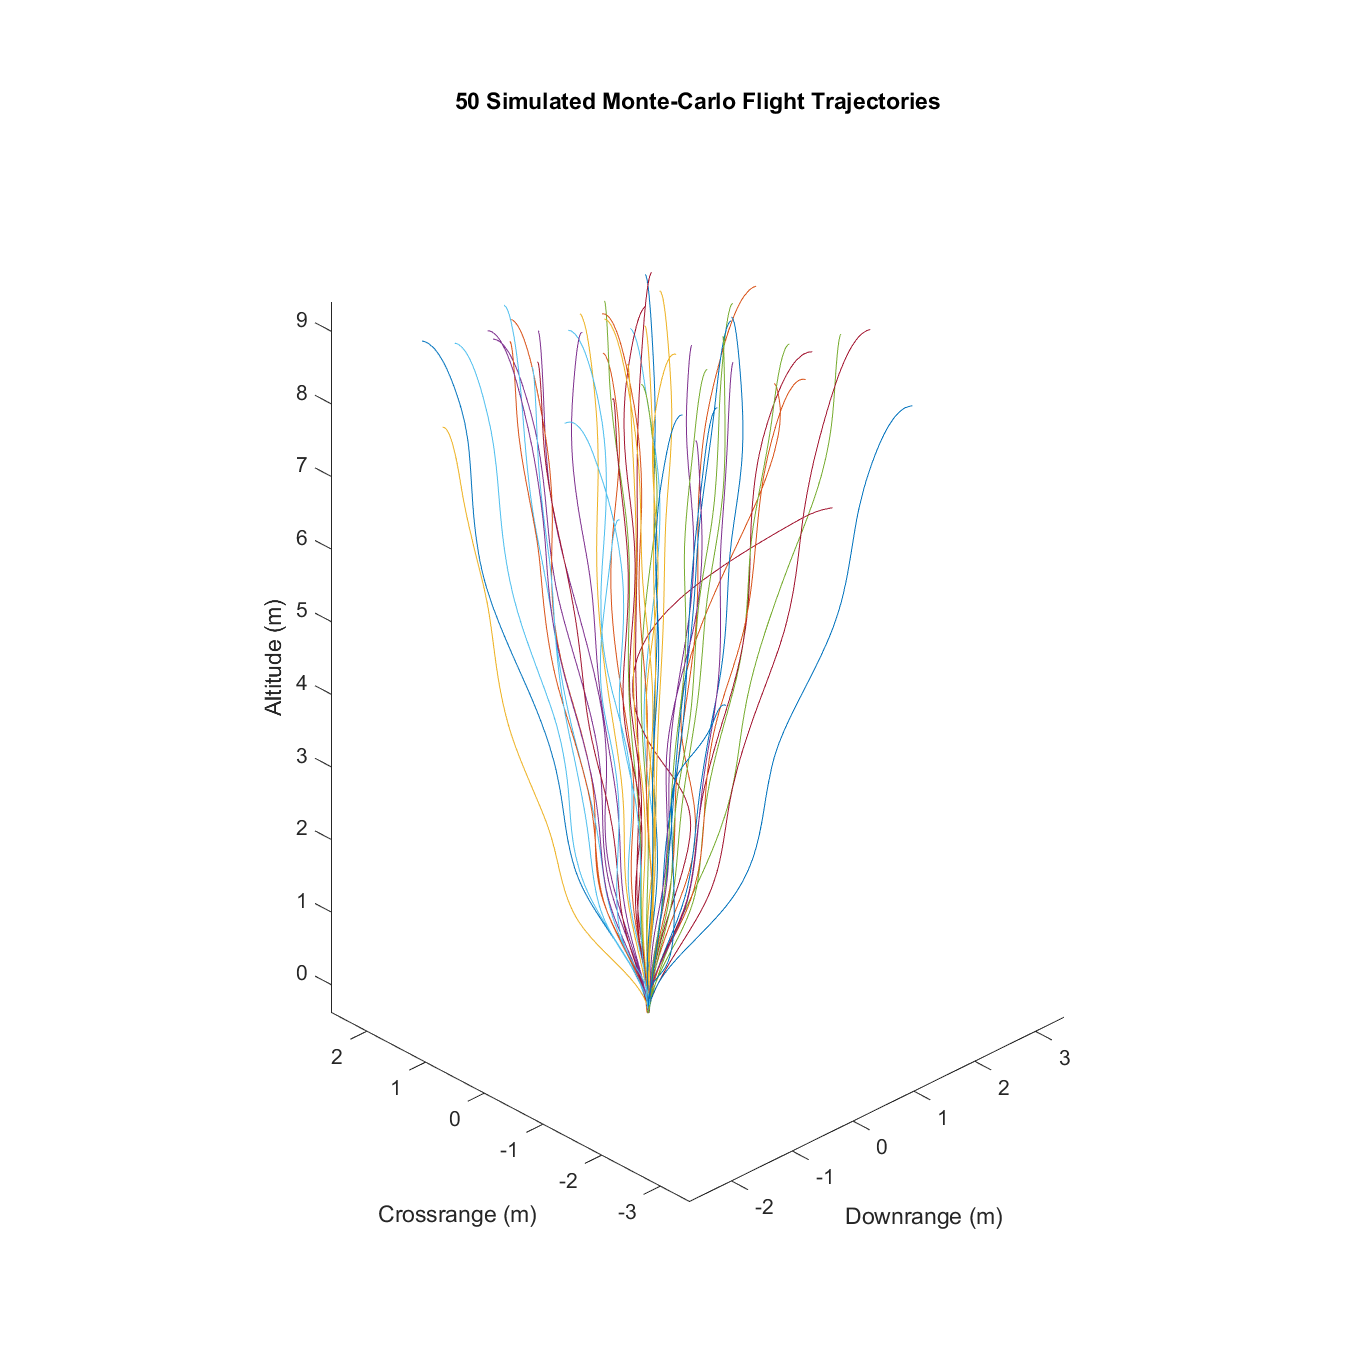
\includegraphics[width=\textwidth]{\Images/rocket_sim/Simu6DOF_60ms.eps}
        \caption*{$T_e = 60 \si{\milli\second}$}
    \end{minipage}%
    \hfill%
    \begin{minipage}[c]{0.48\textwidth}
        \centering
        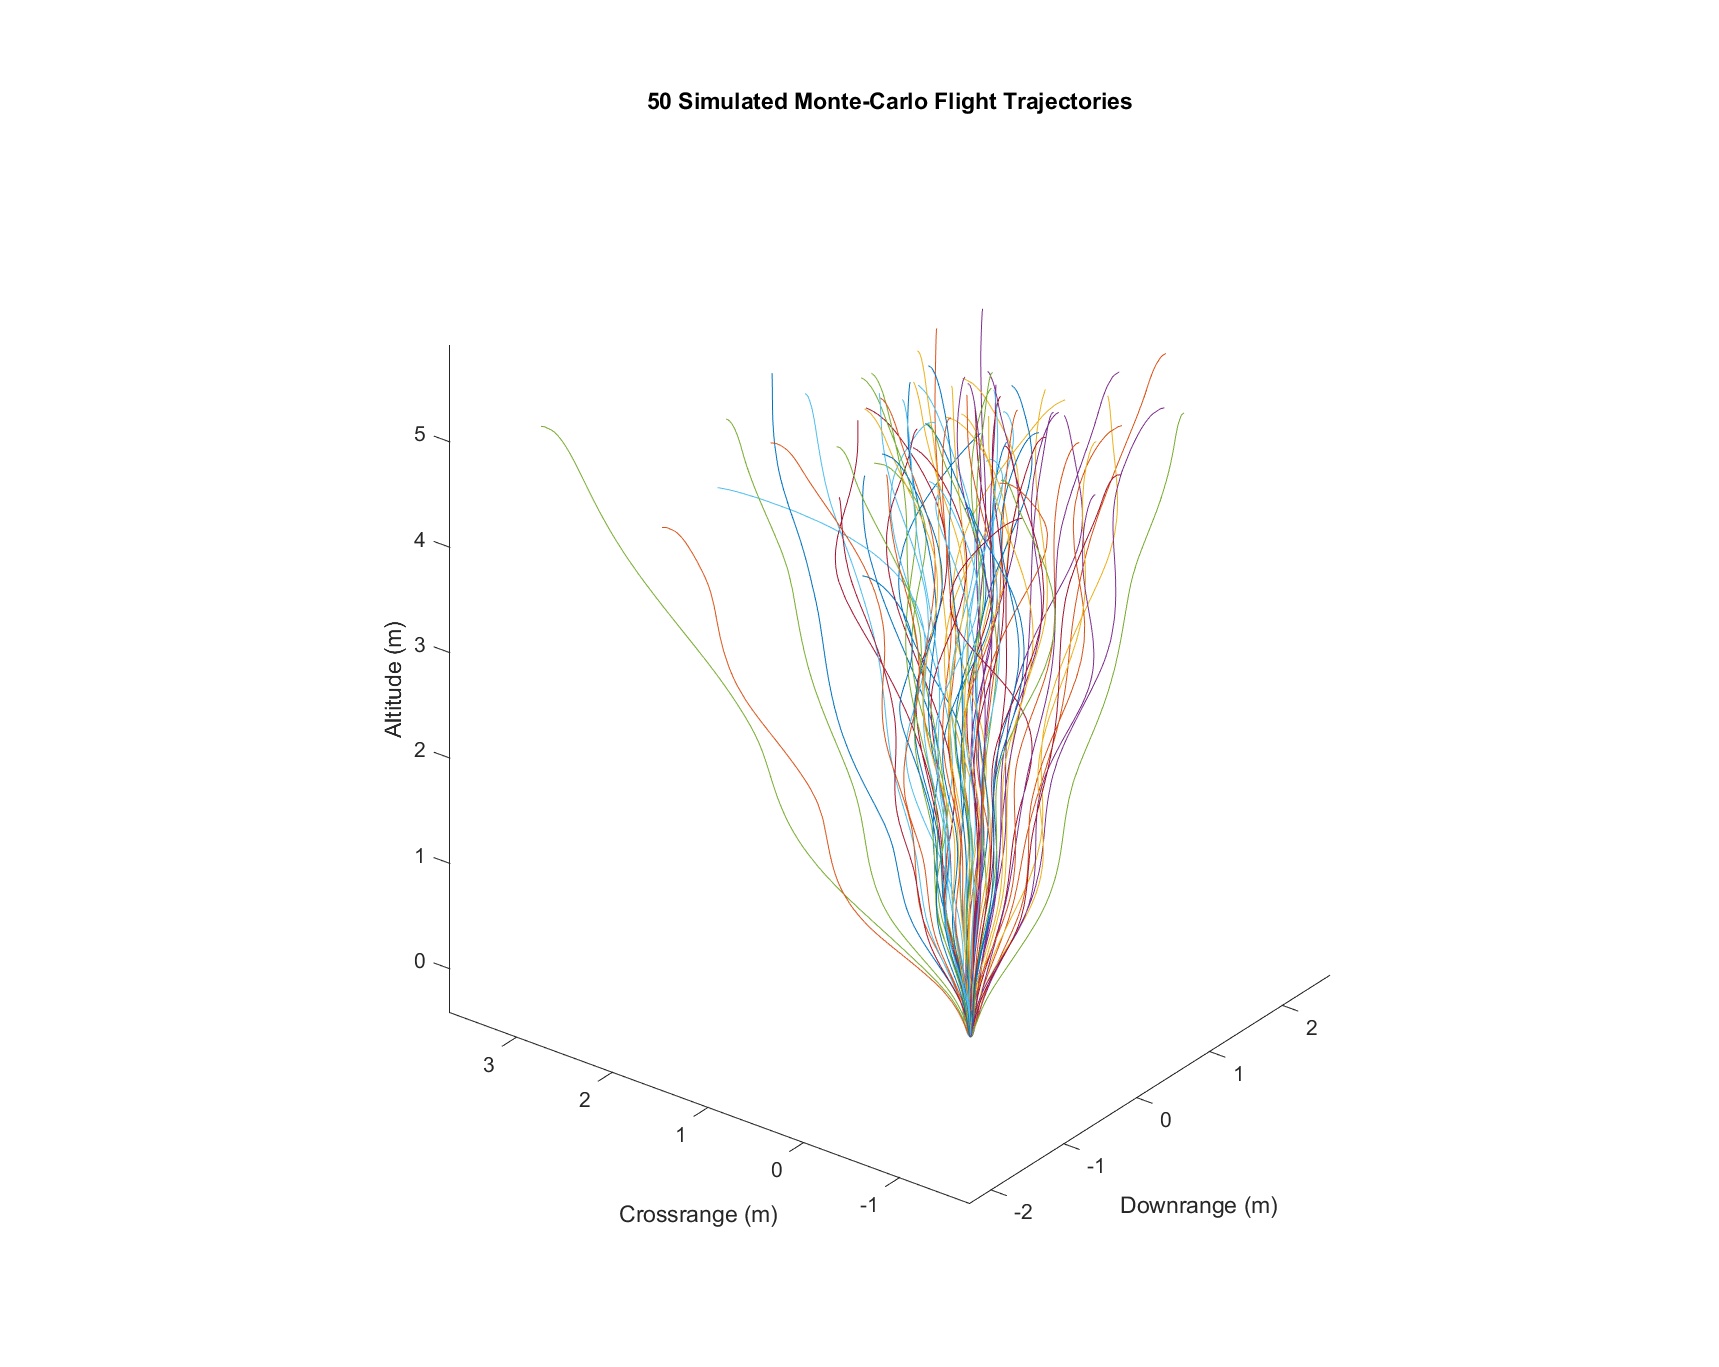
\includegraphics[width=\textwidth]{\Images/rocket_sim/Simu6DOF_80ms.eps}
        \caption*{$T_e = 80 \si{\milli\second}$}
    \end{minipage}%
    \label{img:layout}
\end{figure}

\begin{figure}[!hbt]
    \centering
    \begin{minipage}[c]{0.48\textwidth}
        \centering
        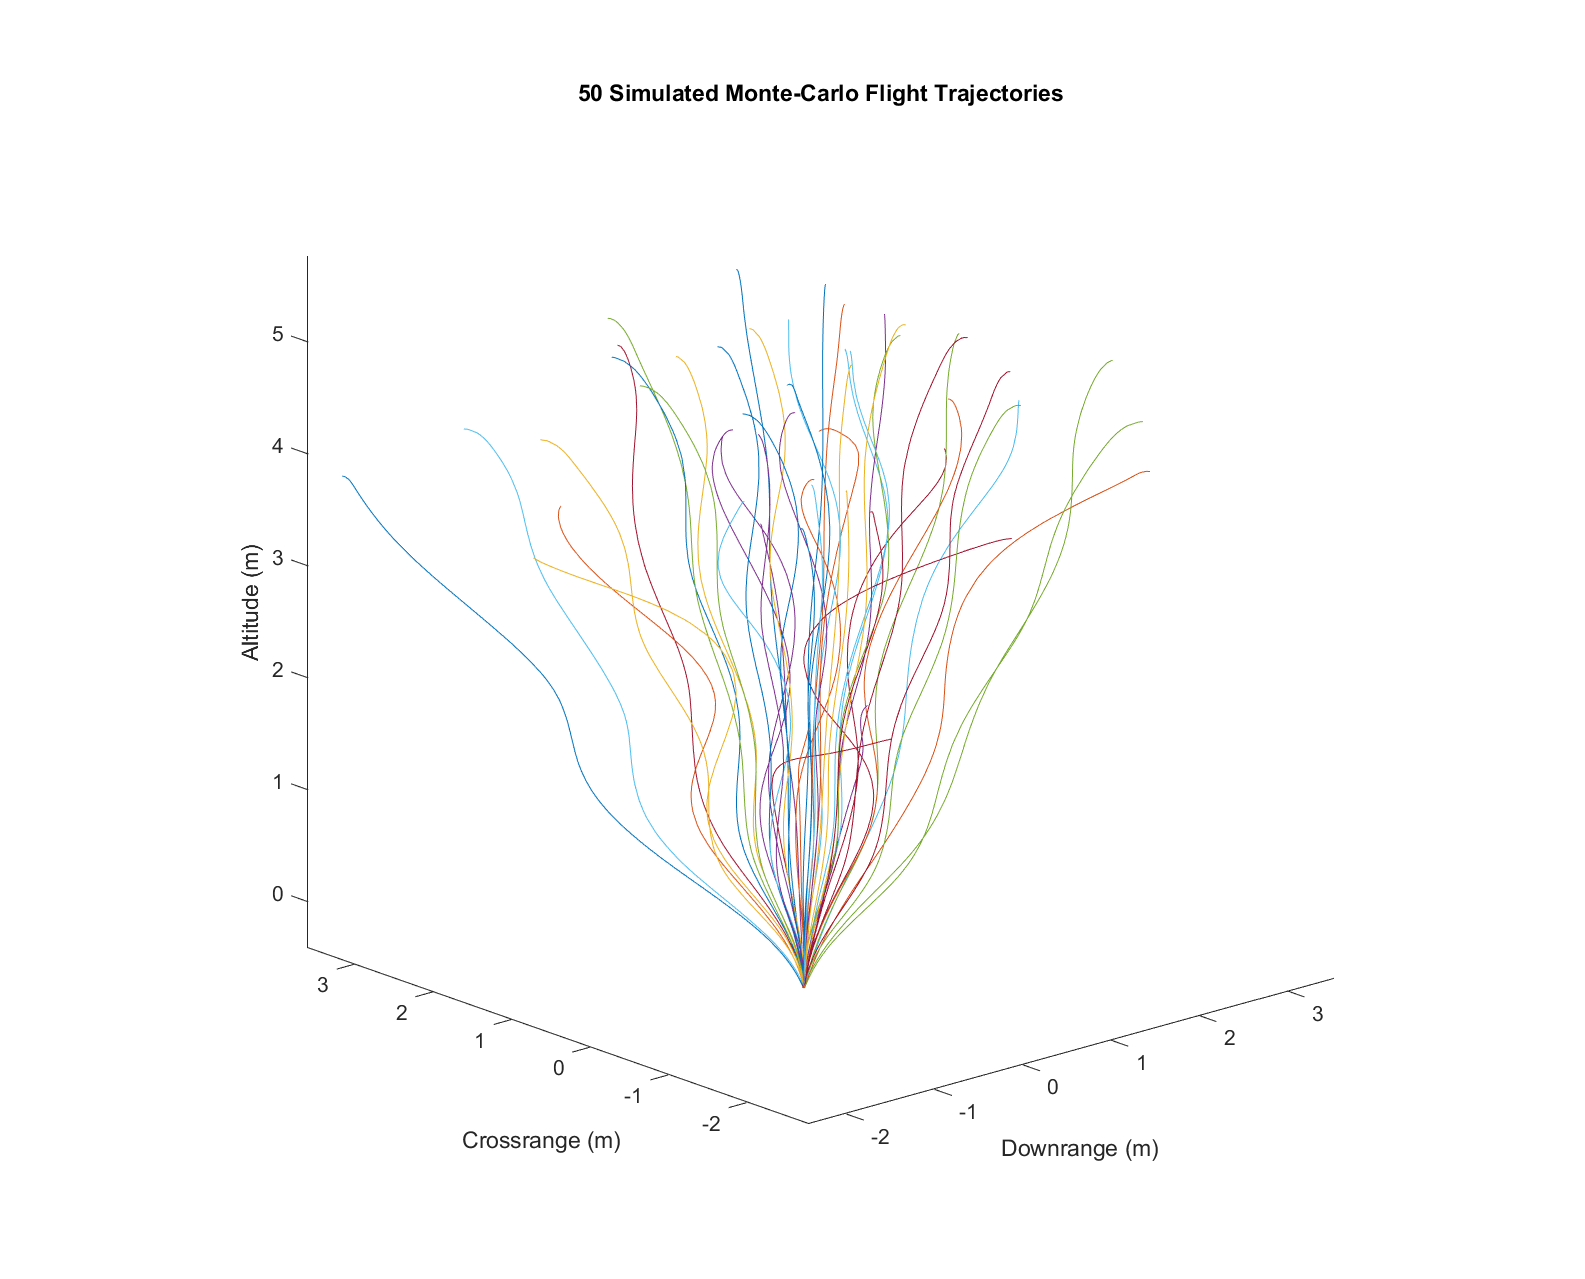
\includegraphics[width=\textwidth]{\Images/rocket_sim/Simu6DOF_100ms.eps}
        \caption*{$T_e = 100 \si{\milli\second}$}
    \end{minipage}%
    \hfill%
    \begin{minipage}[c]{0.48\textwidth}
        \centering
        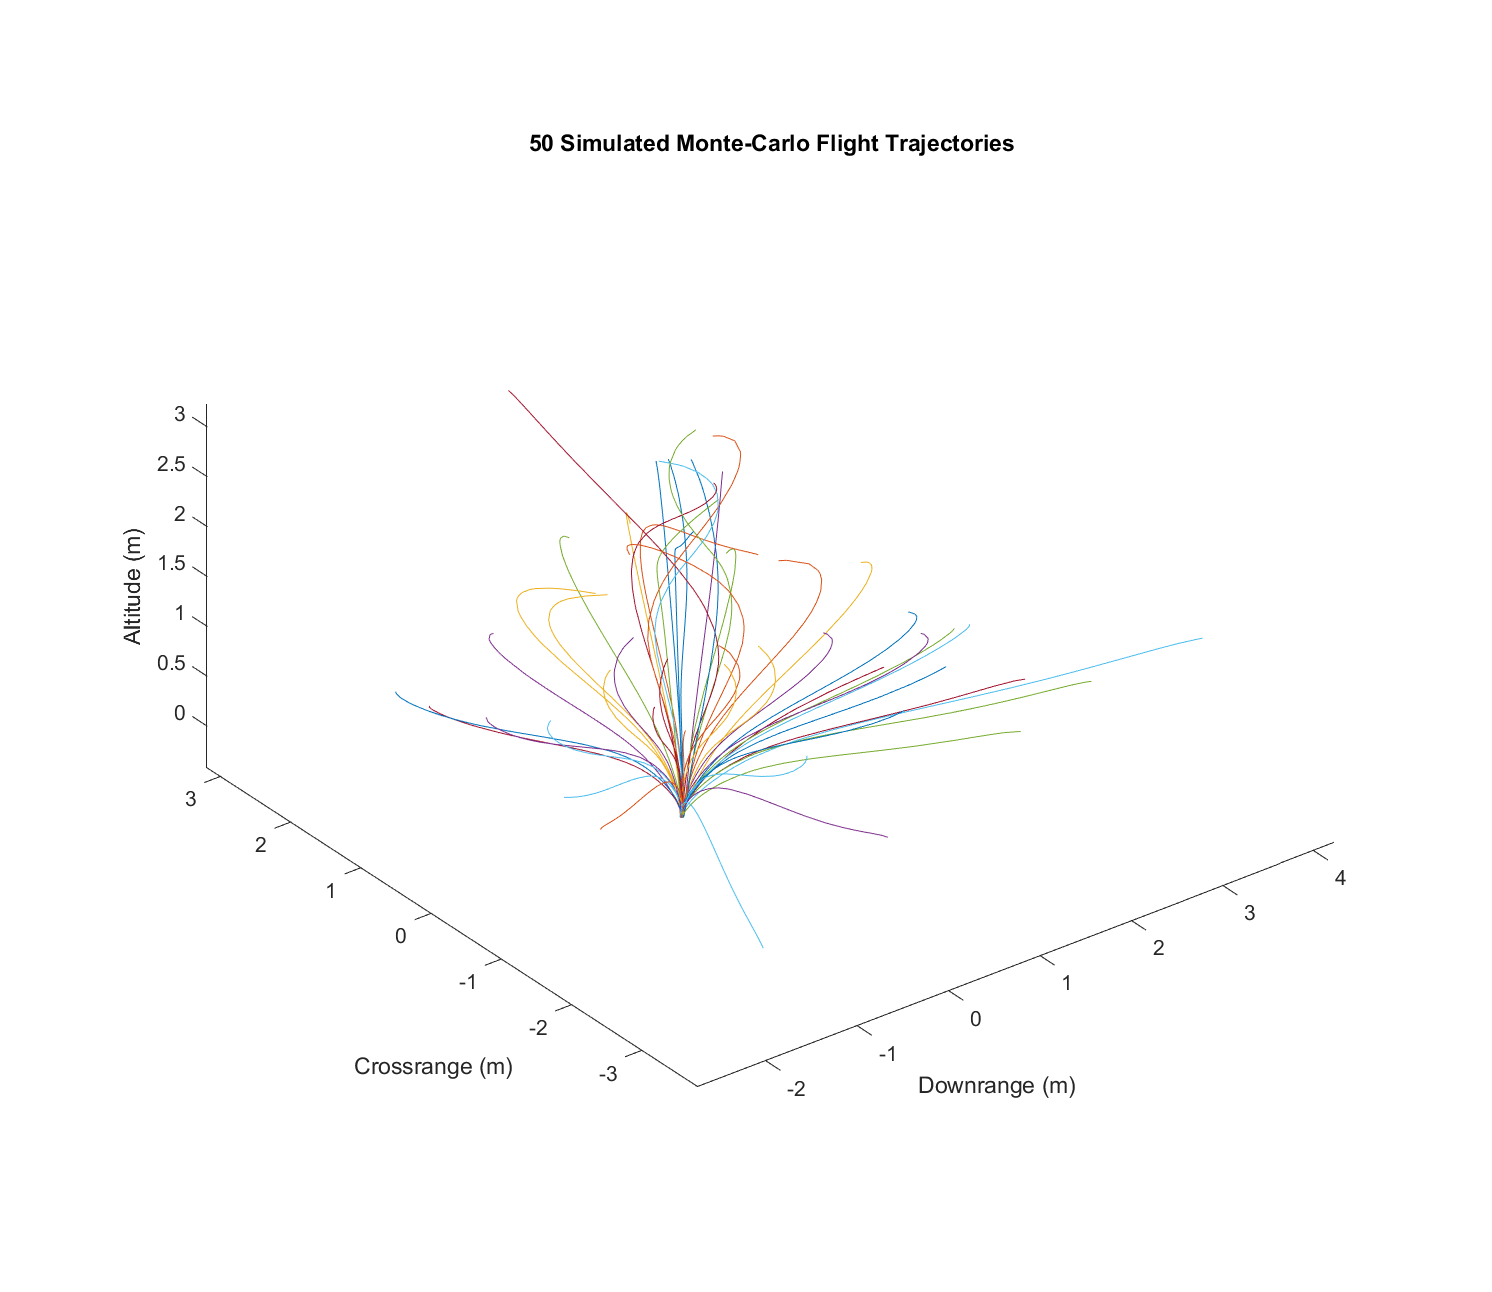
\includegraphics[width=\textwidth]{\Images/rocket_sim/Simu6DOF_500ms.eps}
        \caption*{$T_e = 500 \si{\milli\second}$}
    \end{minipage}%
    \label{img:traj_sim}
    \caption{Trajectory simulations for multiples sampling periods.}
\end{figure}

\FloatBarrier
\chapter{Programmation}\label{annex:prog}
\section{Introduction to devicetrees}\label{sec:dt_intro}
First, we need to explain what is a devicetree, because that's actually far from begin clear and easy to understand.
The wikipedia article describe it concisely, here a quotation :

\begin{quote}
    \quote{In computing, a devicetree (also written device tree)
        is a data structure describing the hardware components of
        a particular computer so that the operating system's kernel
        can use and manage those components, including the CPU or CPUs,
        the memory, the buses and the integrated peripherals.}
    \cite{devicetree}
\end{quote}

\paragraph{}
So, we know that we're going to found some hardware description in theses files. Theses kind of files are
commonly used on the Linux kernel for this purpose, on hardware that is much faster than our small
microcontroller.
This way of describing hardware, even if it's quite difficult to get it rigth enable some extremely smart
options, such as dynamic reconfiguration.

\paragraph{}
In fact, for other controllers we're supposed to bind pins by hand by correctly assigning register values.
This is easy to develop, but once you want to change something, it become difficult to not make mistake by
misreading a value.
This problem is solved with devicetrees, since they store hardware config for ourselves. And, they can
even store multiple configuration, and offer the option to switch at compile time.

It's then possible to develop a devicetree for the development board, and for the final board, and within
one parameter change between them !

\paragraph{}
Devicetrees are written in plain text, and there can be only a single file used for the compilation at
a given time. Theses files use the extension ".dts". This main file contain the root, also named "/",
as any UNIX filesystem. Then, we add "folders", which are named nodes to it. Nodes can be
nested inside others to make the code cleaner. Theses are sometimes called sub-nodes. And inside nodes,
there is some properties, that can be seen as a variable that configure one aspect\footnote{
    Properties can be accessed by the software, thus they may not describe an hardware caracteristic but
    some boundaries imposed by the hardware to the software. This can substitue to \#define macros in plain
    C.
}.

As an example, a node may be RAM, and properties are the size, the speed and any other hardware
parameters.

In correctly designed devicetrees, there shall be one node for each device that can't be detected on
runtime. This include I2C slaves.

\paragraph{}
Each node can get a "compatible" property. This enable a very usefull tool on the compilation step to ensure
our node is well formed. This property is simply a list of required properties, and they're size. That's a
usefull verification tool, because device tree compiler \textit{can't} check for errors. If leaves you in a
state with invalid devicetree files, and near nothing to debug it.

\paragraph{}
We can easily image that theses files will become big, even for simple systems. To give an idea, there is
arround one thousand of lines just for our simple microcontroller !

Thus, the developpers of Device Tree Compilers managed to create an include syntax, based on overlays files
(".dts\textbf{i}"). Theses are included by after and contain only the code for a single peripheral.
Then, we include them over the main devicetree file.

If the new nodes were not present, they're added to the main code. If they were already existing, the new
file will overhide properties.
It's always the latest added that take the priority.


\section{RTOS}
For this second part, we'll go a bit higher in the software structure of the
project, and see the different layers. The first layer is the one we'll
describe here, which is the RTOS.

This stand for Real Time Operating System.

\begin{quote}
    \quote{A real-time operating system (RTOS) is an operating system (OS) for real-time
        computing applications that processes data and events that have critically defined
        time constraints. A RTOS is distinct from a time-sharing operating system, such as
        Unix, which manages the sharing of system resources with a scheduler, data buffers,
        or fixed task prioritization in multitasking or multiprogramming environments. All
        operations must verifiably complete within given time and resource constraints or
        else fail safe. Real-time operating systems are event-driven and preemptive, meaning
        the OS can monitor the relevant priority of competing tasks, and make changes to
        the task priority.}
    \cite{RTOS}
\end{quote}

\paragraph{}
Thus, we're able to specify strict time constraints for different threads. This
is very usefull, since it enable us to ensure the controller, designed for a
specific sampling rate will iterate at a defined speed.

\subsection{Basic RTOS concepts}
To match they're requirements, near all of the RTOS define some basic concepts,
such as :

\begin{itemize}
    \item A scheduler (that may be able to preempt a task)
    \item Some communication protocols :
          \begin{itemize}
              \item Queues
              \item Messages
              \item events
          \end{itemize}
    \item Tasks (which include a priority flag !)
\end{itemize}

\subsubsection{Scheduler}
This is the main aspect of the RTOS, because this the task responsible to
schedule other tasks, while ensuring real times constraints. There's a lot of
different architecture here, each adding it's own set of positives or negatives
aspects.

\subsubsection{Communication protocols}
For this second concepts, we need to present the differents ways to send data
from one task to the other.

Since we're running multiple task in parallel, we can't define which
instruction will be executed before another on another task. Thus, standard
memory transfers, based on variables and pointers become unreliable. In fact,
most of the RTOS block these kind of transfers !\footnote{ The name may be
    different from one RTOS to the other, but the concepts remains the same. Here,
    we used the Zephyr RTOS naming convension, as we used this RTOS by after. }

Thus, we're forced to use thread-safe memory transfers, which are based on
buffers, FIFOs and other principle. Since the RTOS manage these, it can enable,
or disable some operations on the shared buffer. This is done to ensure memory
safety during the execution of the program.

There's indeed multiple type of transfers, depending the needs. The first,
Queues are FIFOs, and able to transfers large amount of data while ensuring the
order. The drawback of them is they're memory footprint which can be quite
large.

The second ones are similar, but only enable a small amount of data to be
transfered. And, as opposed to the FIFOs, when we overwrite the data, it's
deleted rather than pushed on the Queue. It's memory footprint is similar as
the size of a single object, but, it won't enable the conservations of previous
sample. Thus, we may skip data.

The last one are Events, which are simply bit. We flip them, to notify a thread
that something can, or can't be done.

\subsubsection{Tasks}
The last concept is the Task. This correspond to a thread that is going to be
executed on the CPU. For example, a task may be the main as we know.

Since tasks are handled by the RTOS, it's possible to run multiple tasks in
parallel, making control logic simpler. Thus, the timing logic (Timestamps...)
can be removed, and replaced by a delay. The RTOS will then pause the task and
execute another for the required duration.
\section{Zephyr RTOS}
As we seen just before, RTOS may be very usefull to create complex programs on CPUs.
Since we're using Zephyr, let's dig a bit deeper into this RTOS.

\subsection{Configuration}
As we seen previously, Zephyr isn't based on pure code to configure the device. It used 
a lot of others files, including devicetrees to describe the hardware.

This image represent the different steps to build an executable image for our chip
\begin{figure}[!hbt]
    \centering
    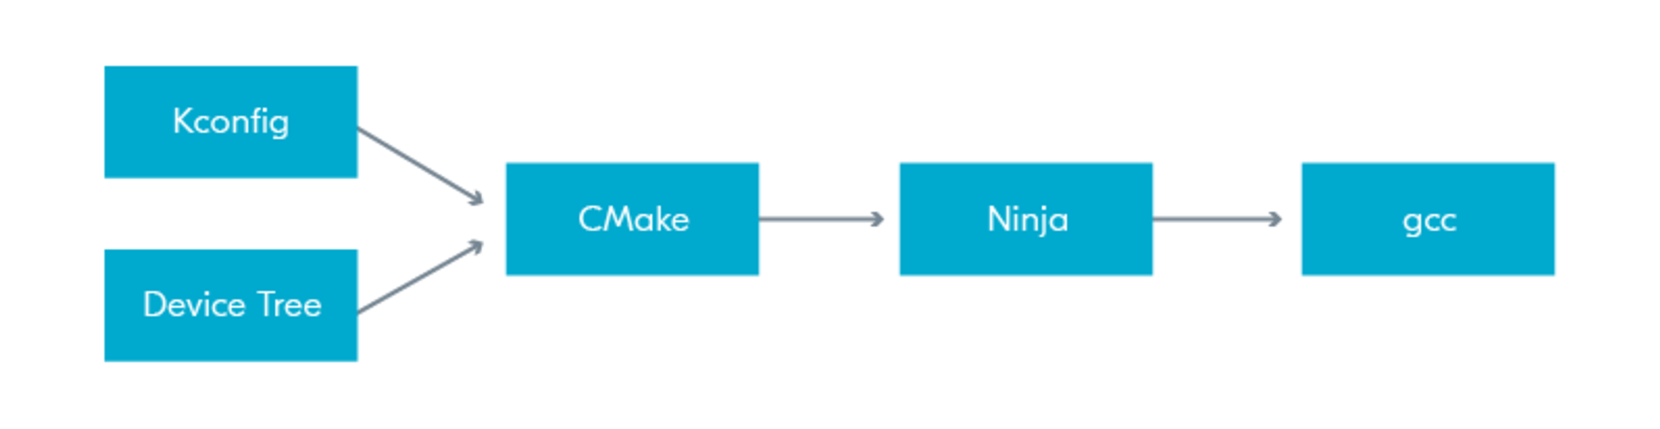
\includegraphics[width=\SchematicWidth]{\Images/Zephyr/ZephyrBuild.eps}
    \caption{Thread management on the Zephyr RTOS}
\end{figure}
\FloatBarrier

In this image, KConfig refer to the software configuration files, that include 
drivers selections and so. This file is linked to the devicetree, because to 
exploit a peripheral, we need to enable it in hardware, but we also need the associated
drivers with it.

To give an example, this kind of files look like : 
\inputminted[linenos, firstline=32, lastline=70]{kconfig}{\Conf/prj.conf}

Thats basically a list of variable that we set to enable, or disable a software driver.

\subsection{Tasks management}
Zephyr does the task management in a different way other RTOS would. It is not bound to 
the fixed interval timer that would trigger a scheduling every period. This RTOS use the
task as self-scheduling.

\begin{figure}[!hbt]
    \centering
    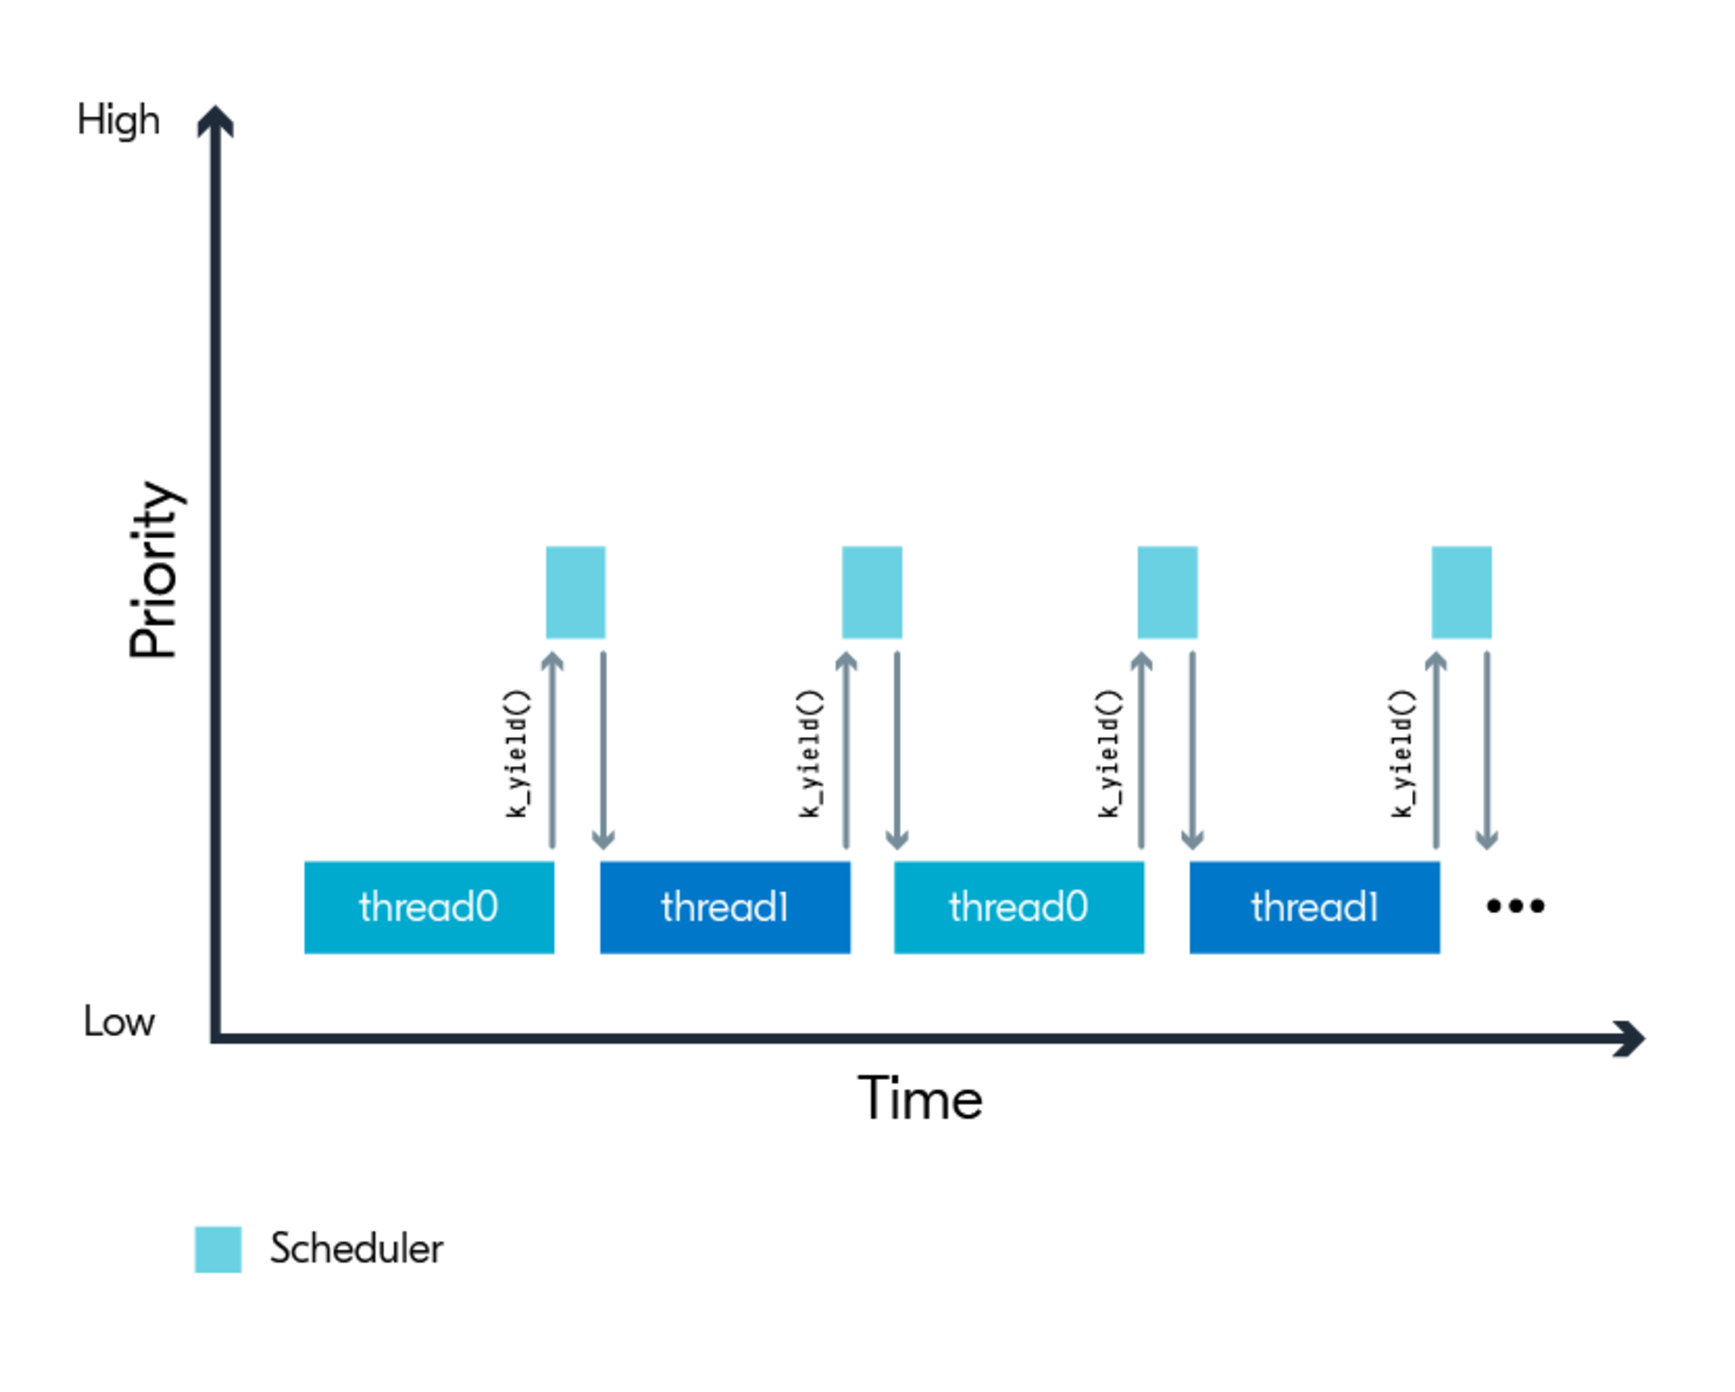
\includegraphics[width=\SchematicWidth]{\Images/Zephyr/ThreadMGNT.eps}
    \caption{Build chain for Zephyr RTOS}
\end{figure}
\FloatBarrier

As we may see on this image, that came from the Nordic training center \cite{NordicFundamentals} 
and \cite{NordicAdvanced} courses, the scheduler is called once a task enter a delay state, or 
yield itself.

On another hand, the RTOS include a safety timer, set to ten milliseconds that will force the
scheduler to be called. This ensure, even if a task enter an infinite loop, or crash, that
the others tasks wont crash.

\subsection{Final words}
To conclude on this RTOS part, we've seen the most basic concepts, but that's enough to
understand how our project is build, and how code interract with other code.

To sum up, Zephyr is an RTOS, used to manage a lot of different things on the project, 
from the most basic configuration of the hardware to the tasks management during the 
execution.


\end{document}
